% TODO: Cite maps
% TODO: Add section about `botplot`

\section{Results}
\label{sec:results}
This section presents the results of simulations meant to determine the performance of the developed search algorithms. Algorithms were run on two maps: Depot {\color{red} [CITE]} and Warehouse {\color{red} [CITE]}. \Cref{fig:bench-maps} shows the maps, with differing denseness of obstacles, used during testing. \\

Search algorithms are evaluated in terms of two key metrics: map coverage over time and computational expense. It is assumed that a higher coverage over time metric would lead to a shorter time to find a search item. Additionally, the consistency between the two simulation environments, \texttt{simple\_sim} and the Gazebo ROS 2 setup is evaluated to confirm the robustness and portability of the behavior implementations.

\begin{figure}[H]
  \centering
  \begin{subfigure}[b]{0.46\textwidth}
    \centering
    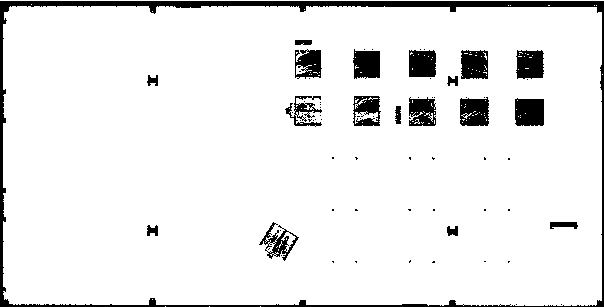
\includegraphics[width=\textwidth]{./figures/depot.png}
    \caption{Depot. Dimensions: 30.2 m by 15.3 m.}
  \end{subfigure}
  \hfill
  \begin{subfigure}[b]{0.46\textwidth}
    \centering
    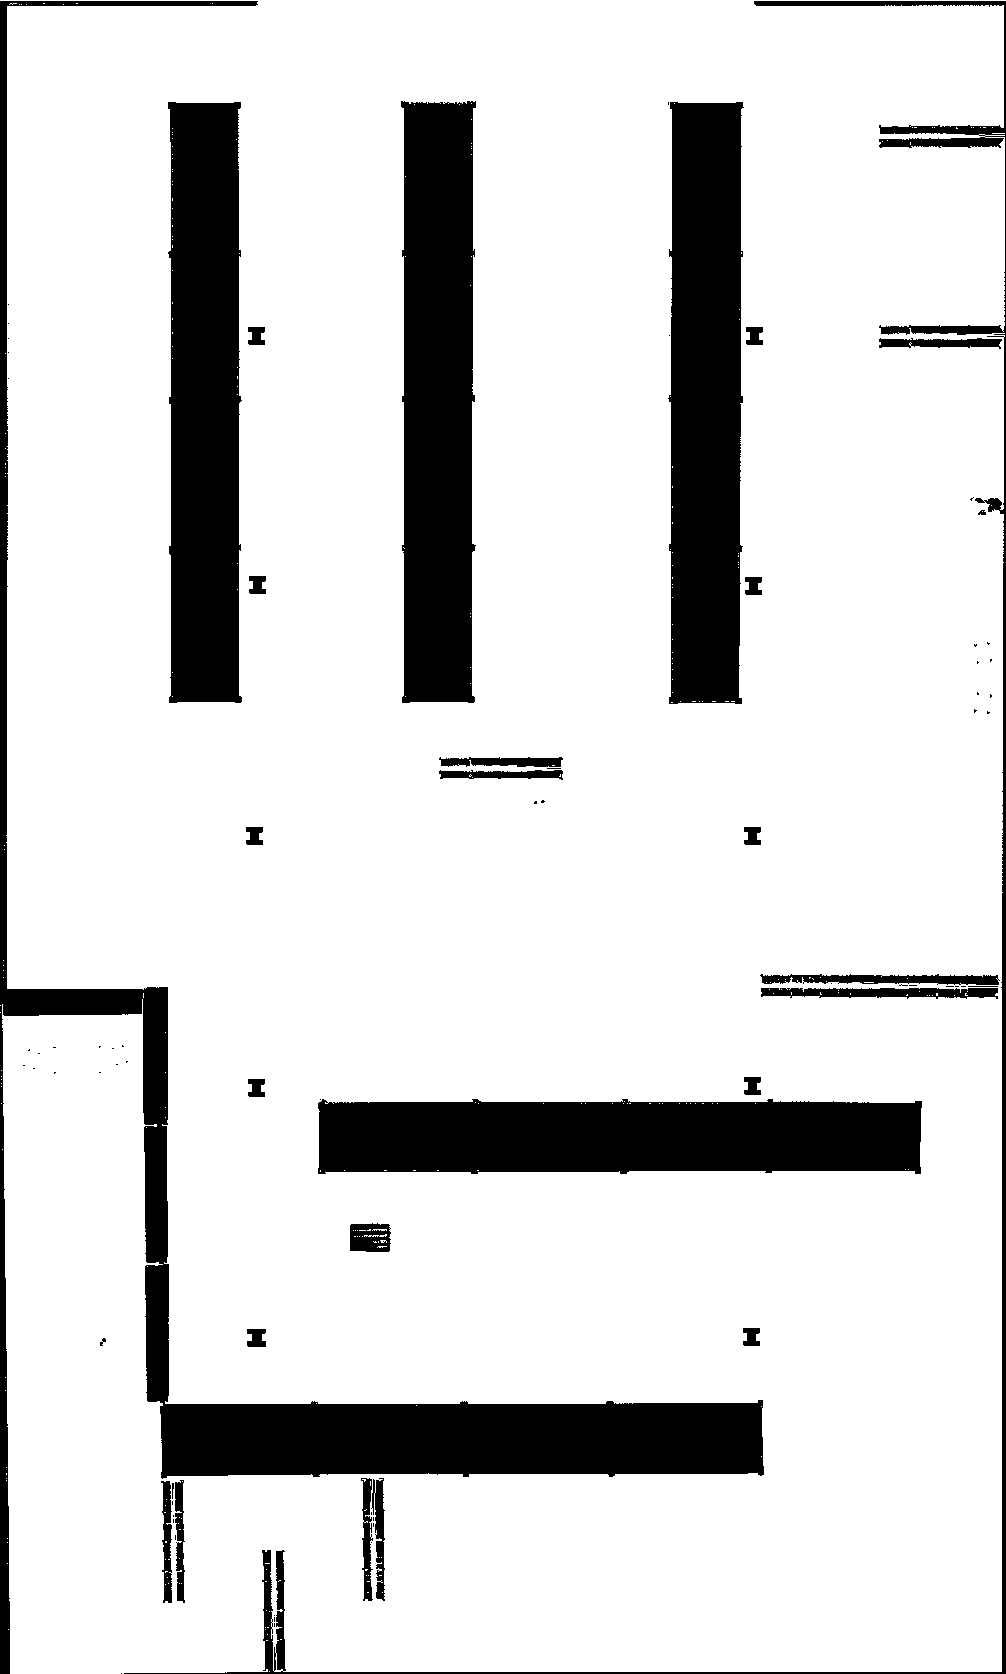
\includegraphics[height=\textwidth, angle=90]{./figures/warehouse.png}
    \caption{Warehouse. Dimmensions: 50.2 m by 30.2 m.}
  \end{subfigure}
  \caption{Maps used for benchmarking search algorithms. The Depot map is smaller and more open compared to the Warehouse map, which is larger and has more hard to reach areas.}
  \label{fig:bench-maps}
\end{figure}

\subsection{Simulator Consistency}
\label{sec:simulator-consistency}
A central goal of the dual-simulator setup is to ensure that algorithms implemented using the \texttt{botbrain} interface yield consistent behavior across both simulators. While Gazebo includes more realistic physics and non-deterministic behavior due to its time step and sensor noise, consistency in qualitative behavior (e.g., coverage trend) is still expected.

\subsubsection{Movement Calibration}
To verify basic motion consistency, simple movement behaviors were executed in both simulators. Speed and steer commands were scaled to get the paths shown in \cref{fig:movement-consistency}. 

\begin{figure}[H]
  \centering
  \begin{subfigure}[b]{0.45\textwidth}
    \centering
    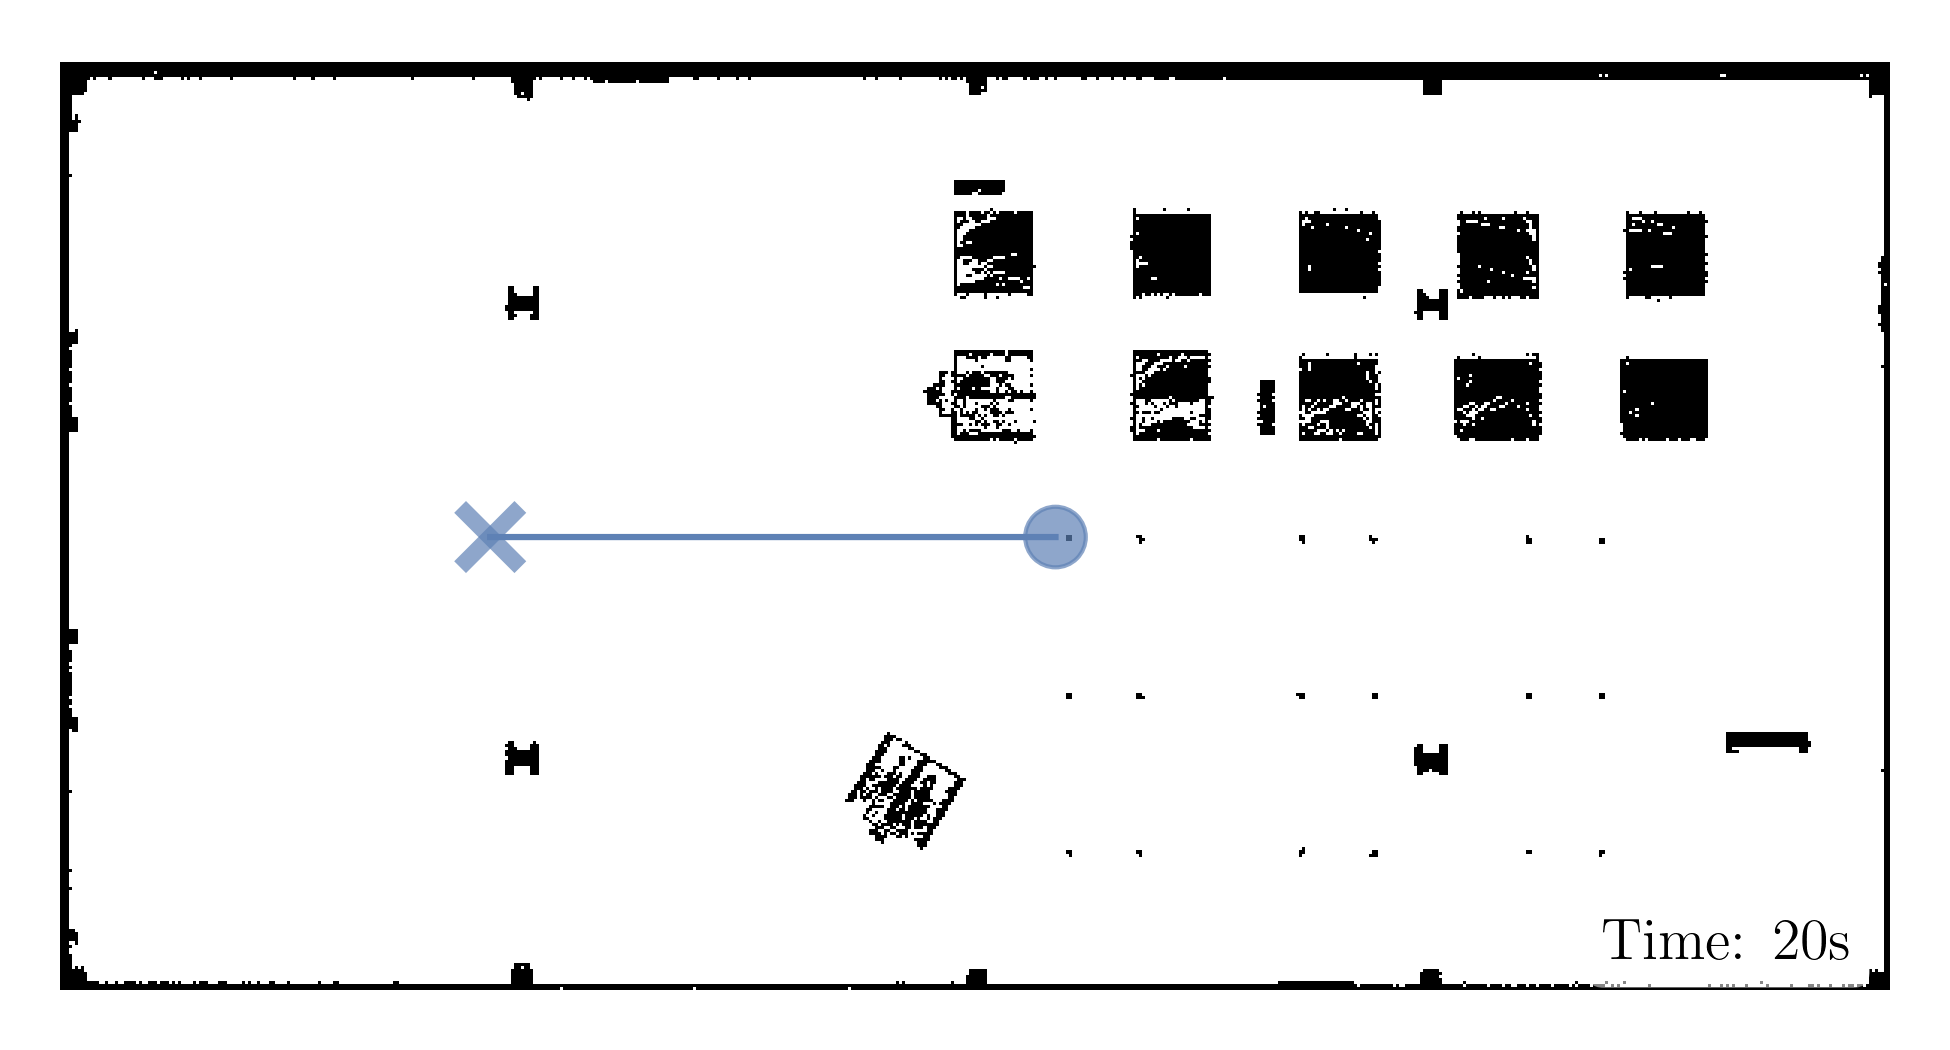
\includegraphics[width=\textwidth]{./figures/plots/consistency/simple-sim-paths-straight.png}
    \caption{\texttt{simple\_sim} straight line.}
  \end{subfigure}
  \begin{subfigure}[b]{0.45\textwidth}
    \centering
    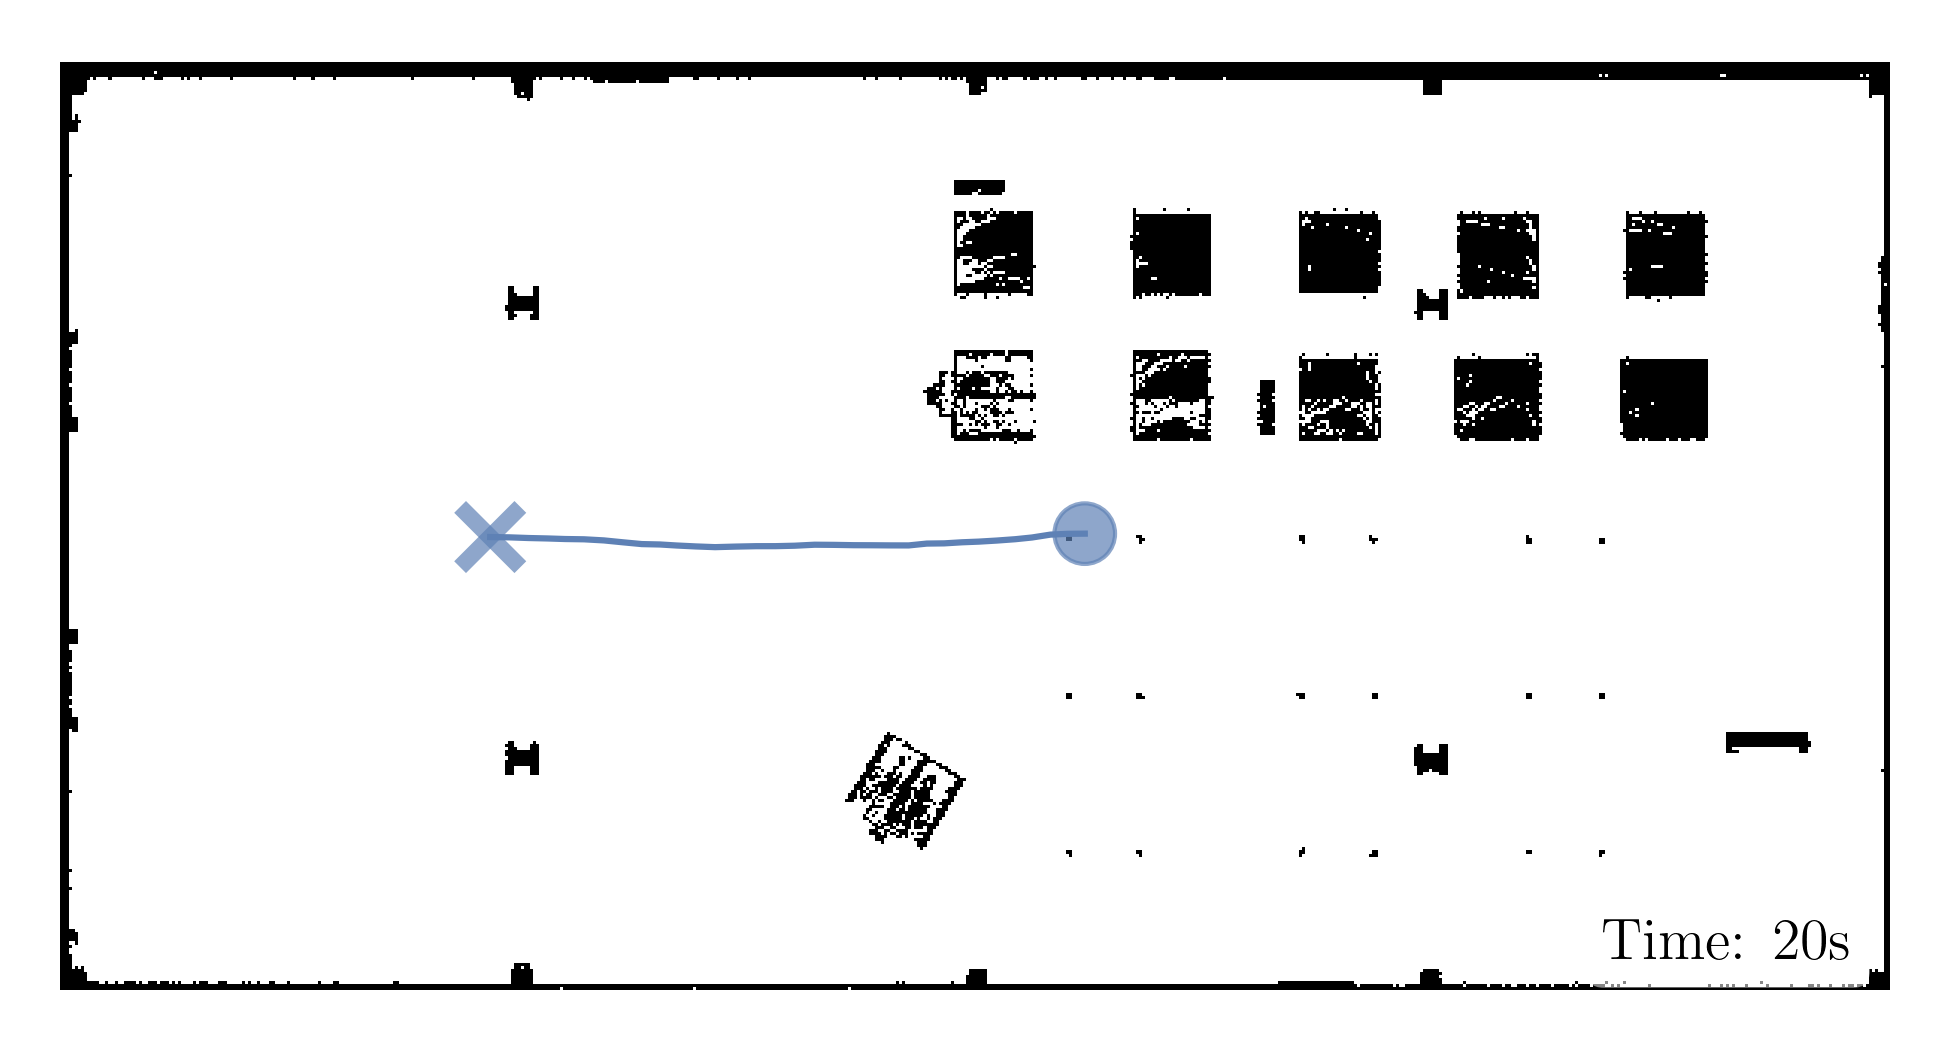
\includegraphics[width=\textwidth]{./figures/plots/consistency/ros-2-paths-straight.png}
    \caption{ROS 2 Gazebo straight line.}
  \end{subfigure}\\
  \begin{subfigure}[b]{0.45\textwidth}
    \centering
    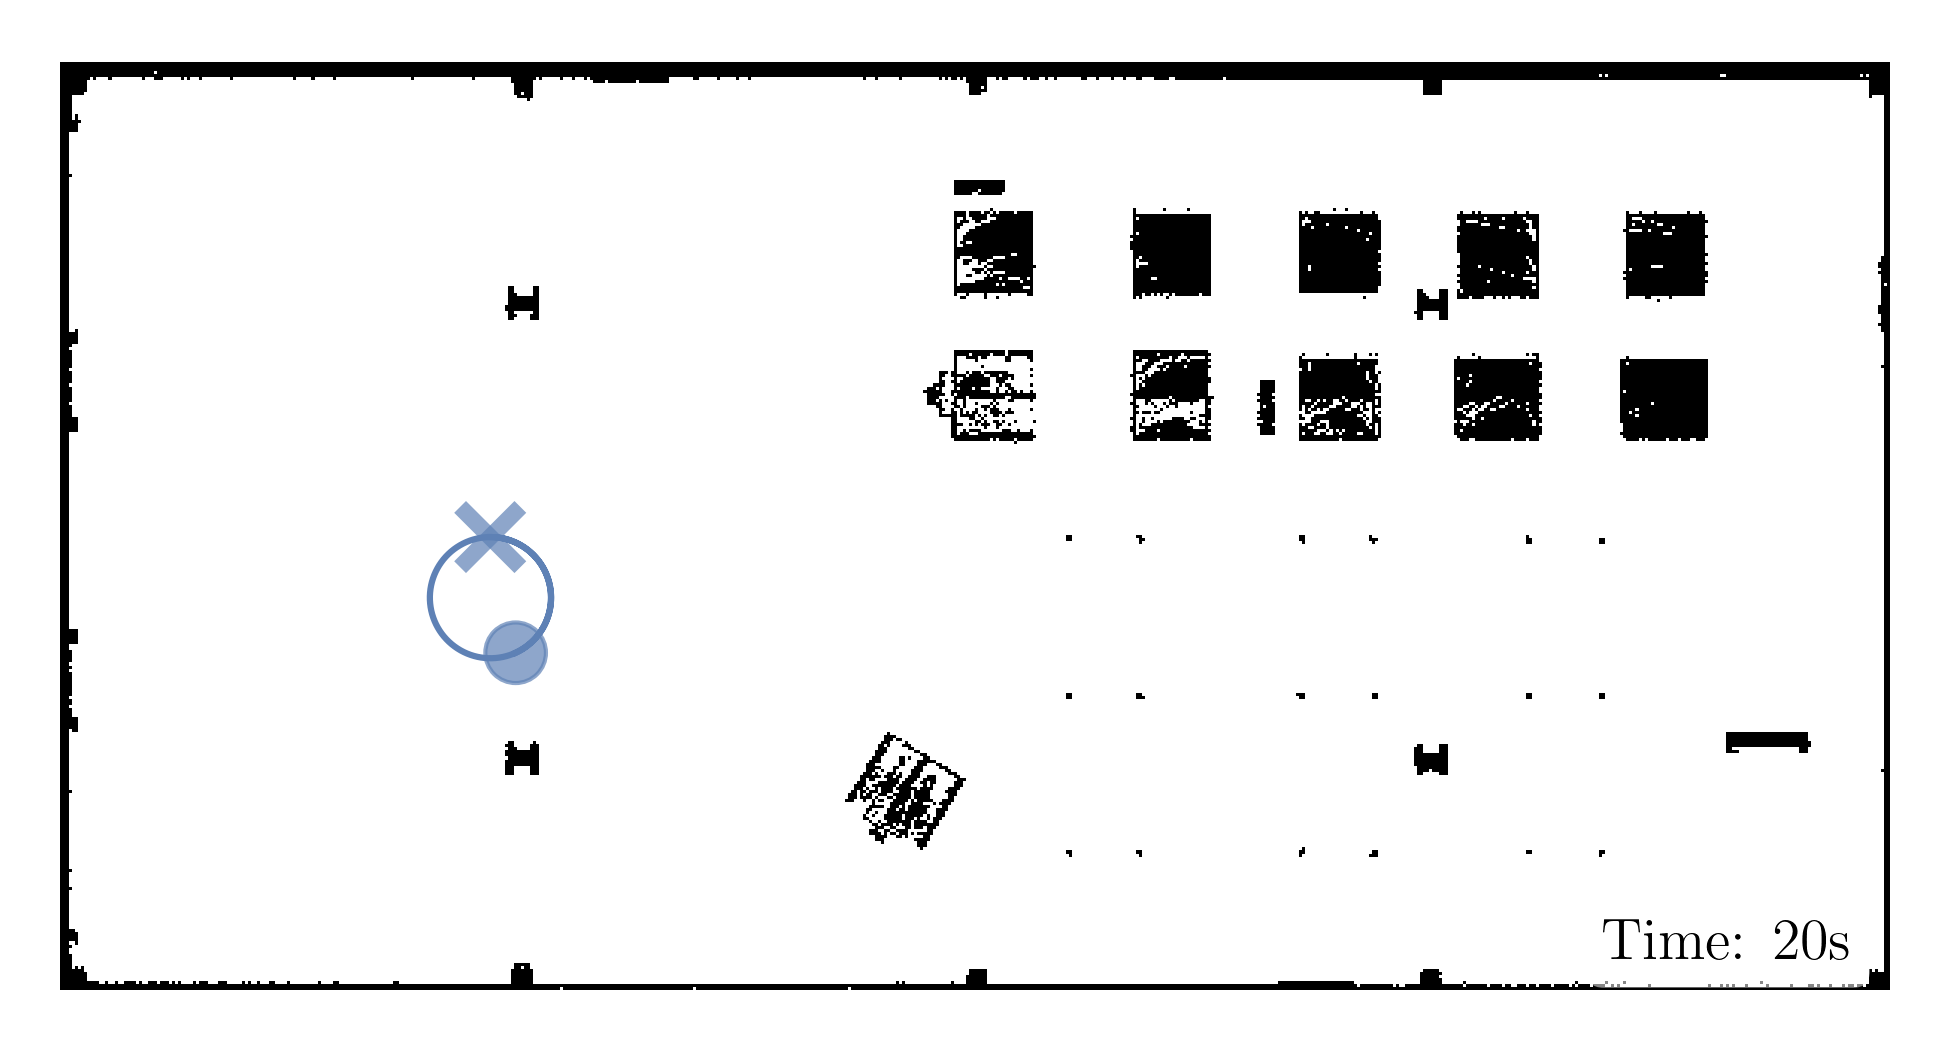
\includegraphics[width=\textwidth]{./figures/plots/consistency/simple-sim-paths-circle.png}
    \caption{\texttt{simple\_sim} circular.}
  \end{subfigure}
  \begin{subfigure}[b]{0.45\textwidth}
    \centering
    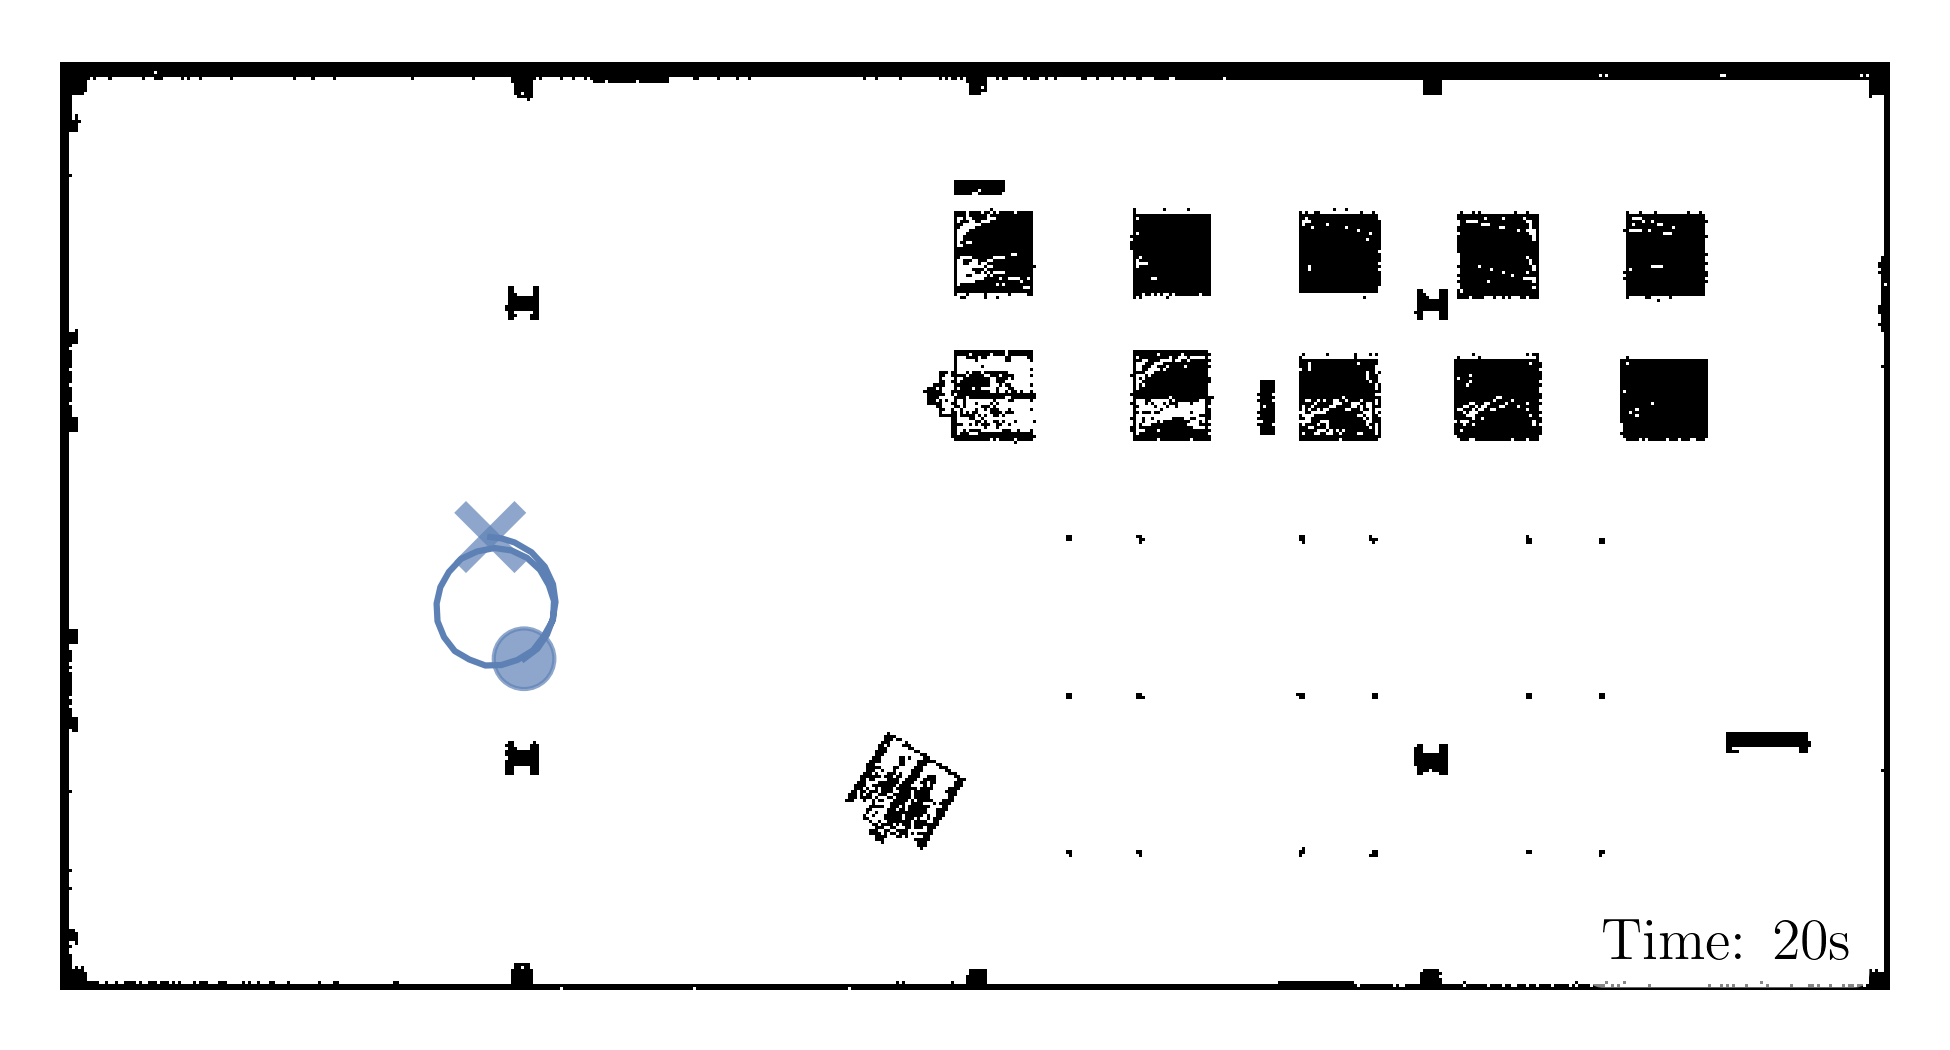
\includegraphics[width=\textwidth]{./figures/plots/consistency/ros-2-paths-circle.png}
    \caption{ROS 2 Gazebo circular.}
  \end{subfigure}
  \caption{Paths produced by \texttt{simple\_sim} and ROS 2 Gazebo.}
  \label{fig:movement-consistency}
\end{figure}

The paths are visually similar, indicating that the velocity commands generated by the behavior logic are interpreted consistently across both environments.

\subsubsection{Performance Consistency}
To validate performance characteristics across simulators, the coverage of 4 robots was recorded over 6 runs for the behaviors developed in \cref{sec:search-algorithms} in both simulators. \Cref{fig:coverage-benchmark-all} shows the results of this test.

% TODO: Fix "Diff." and "Diference"
\begin{figure}[H]
    \centering
    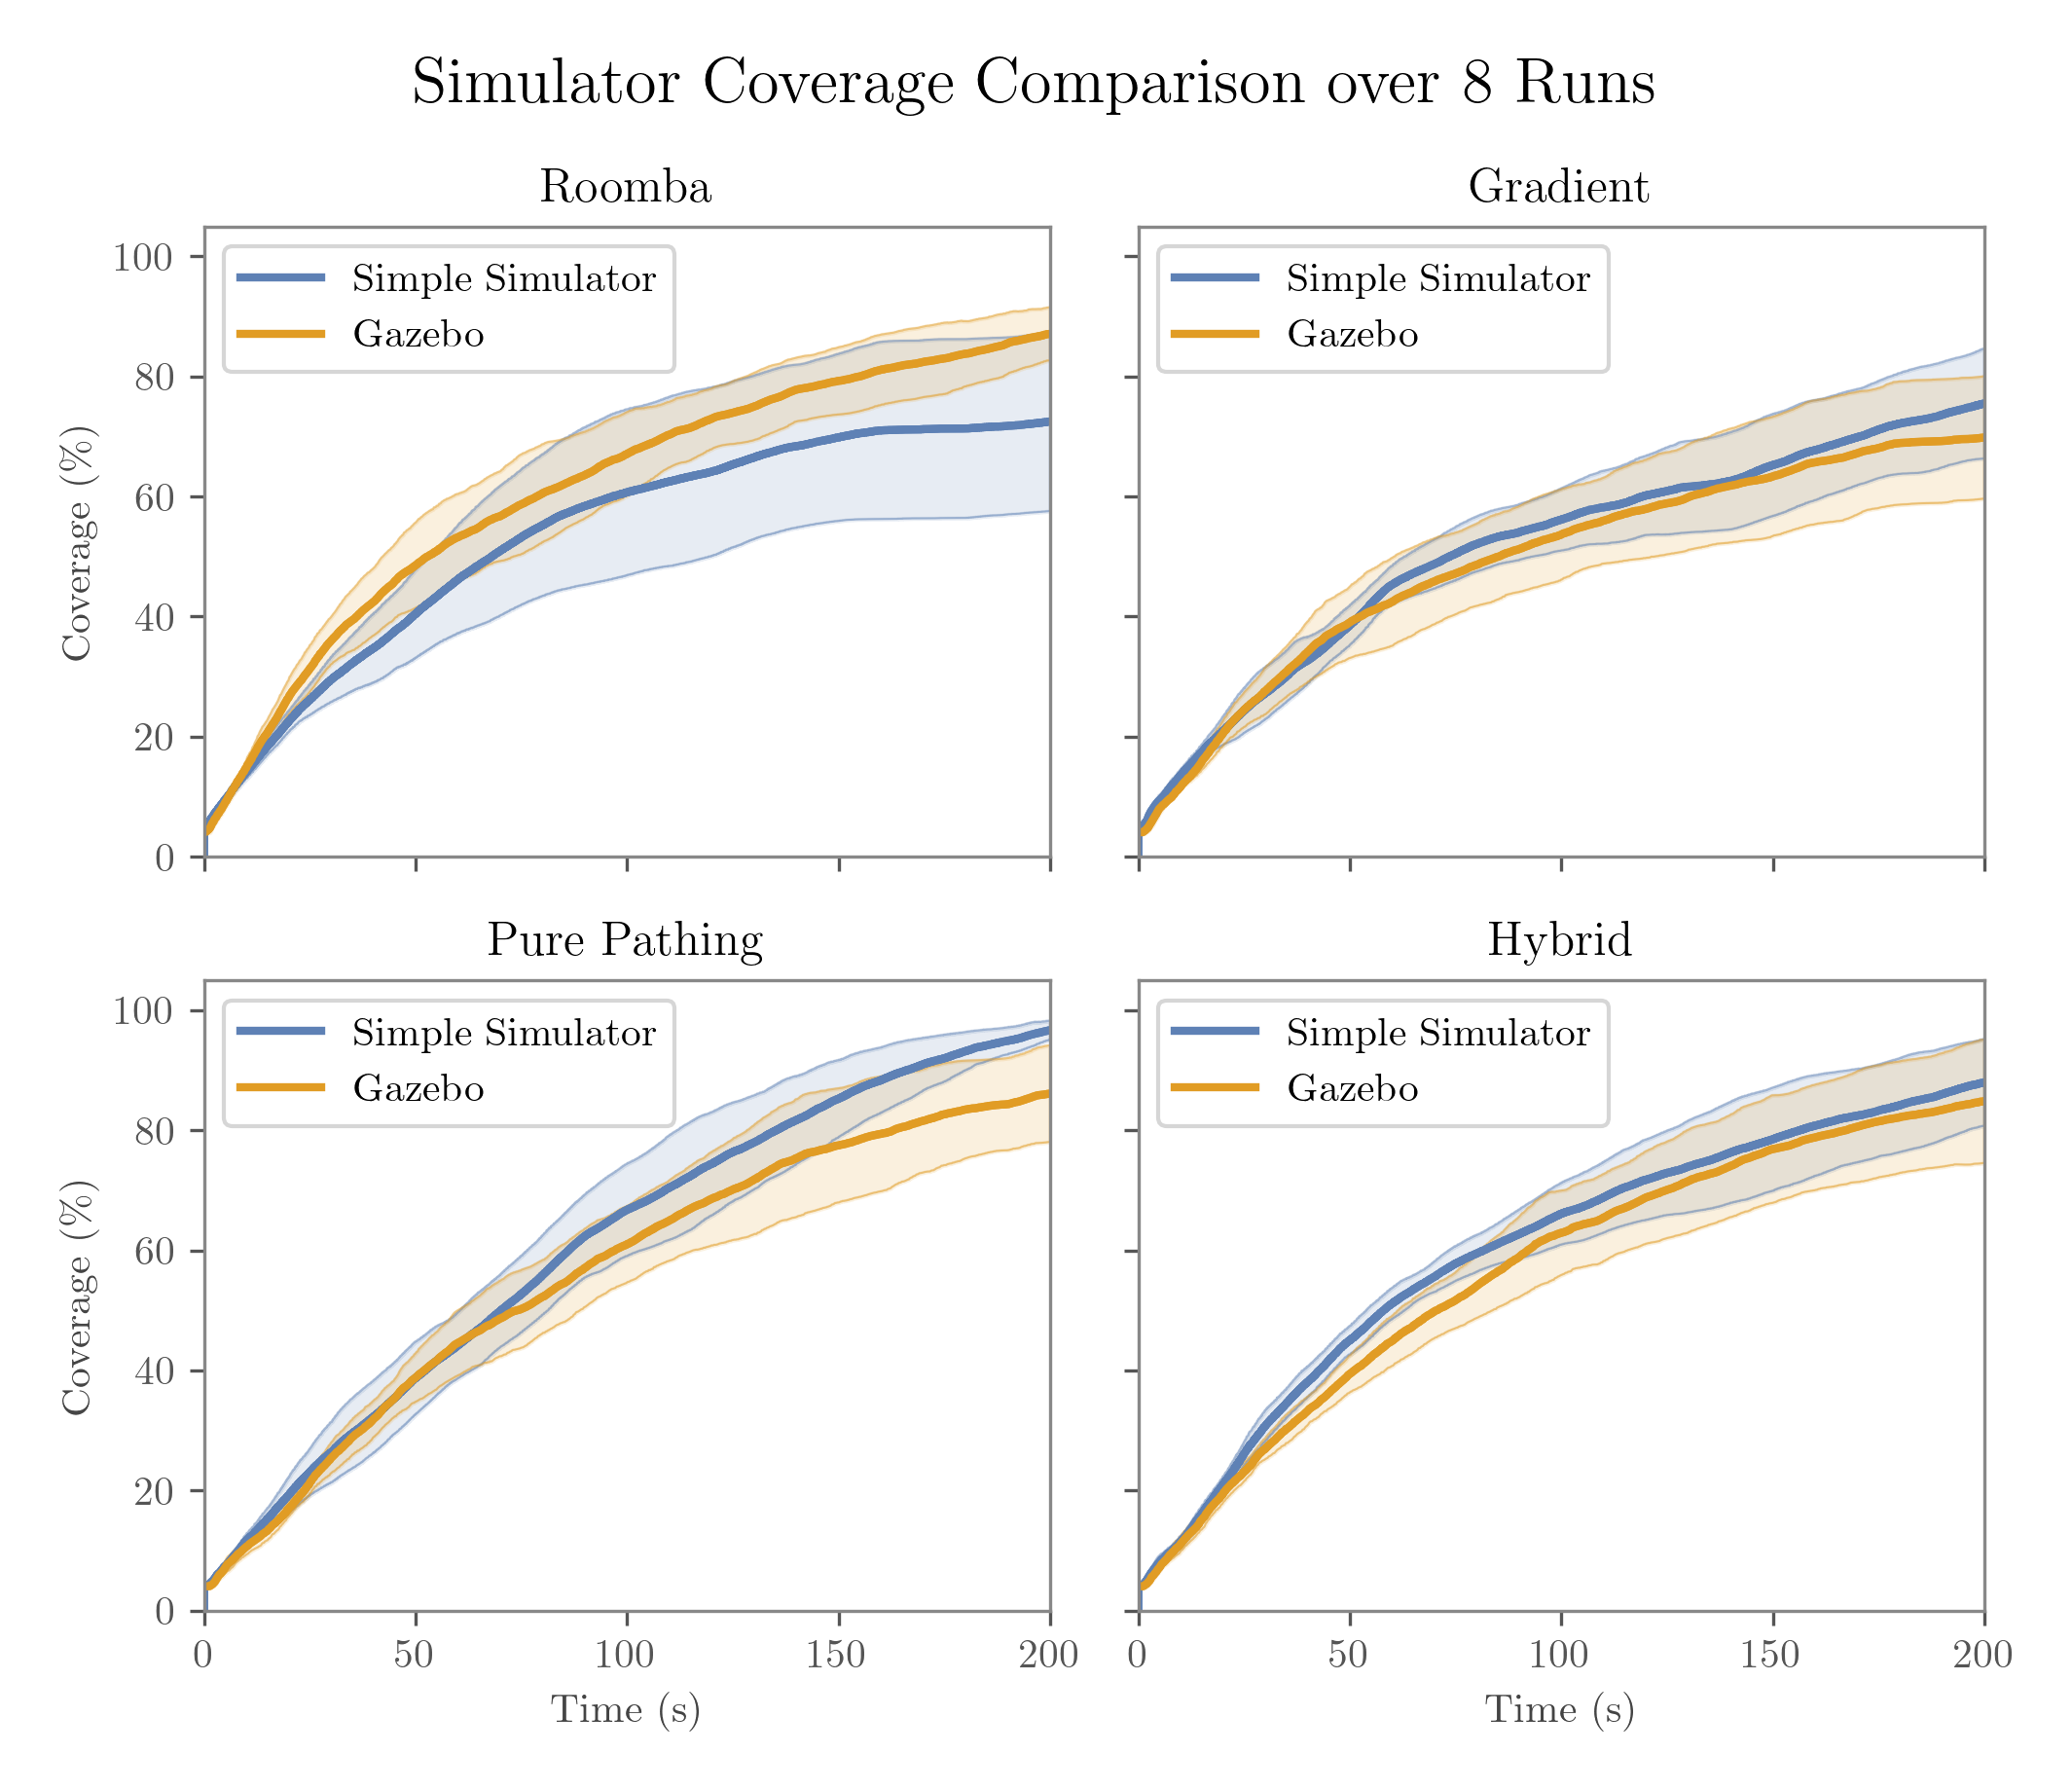
\includegraphics[width=0.95\textwidth]{./figures/plots/consistency/gazebo_vs_simple_sim_coverage.png}
    \caption{Comparison of coverage over time between ROS 2 Gazebo and \texttt{simple\_sim}.}
    \label{fig:coverage-benchmark-all}
\end{figure}

The coverage performance seems to match well between the two simulators, with coverage mostly staying within 1 standard deviation of each other. The Roomba algorithm does, however, seem to perform better in the gazebo environment. \Cref{fig:coverage-benchmark-diff} shows the difference in coverage performance.

\begin{figure}[H]
    \begin{center}
        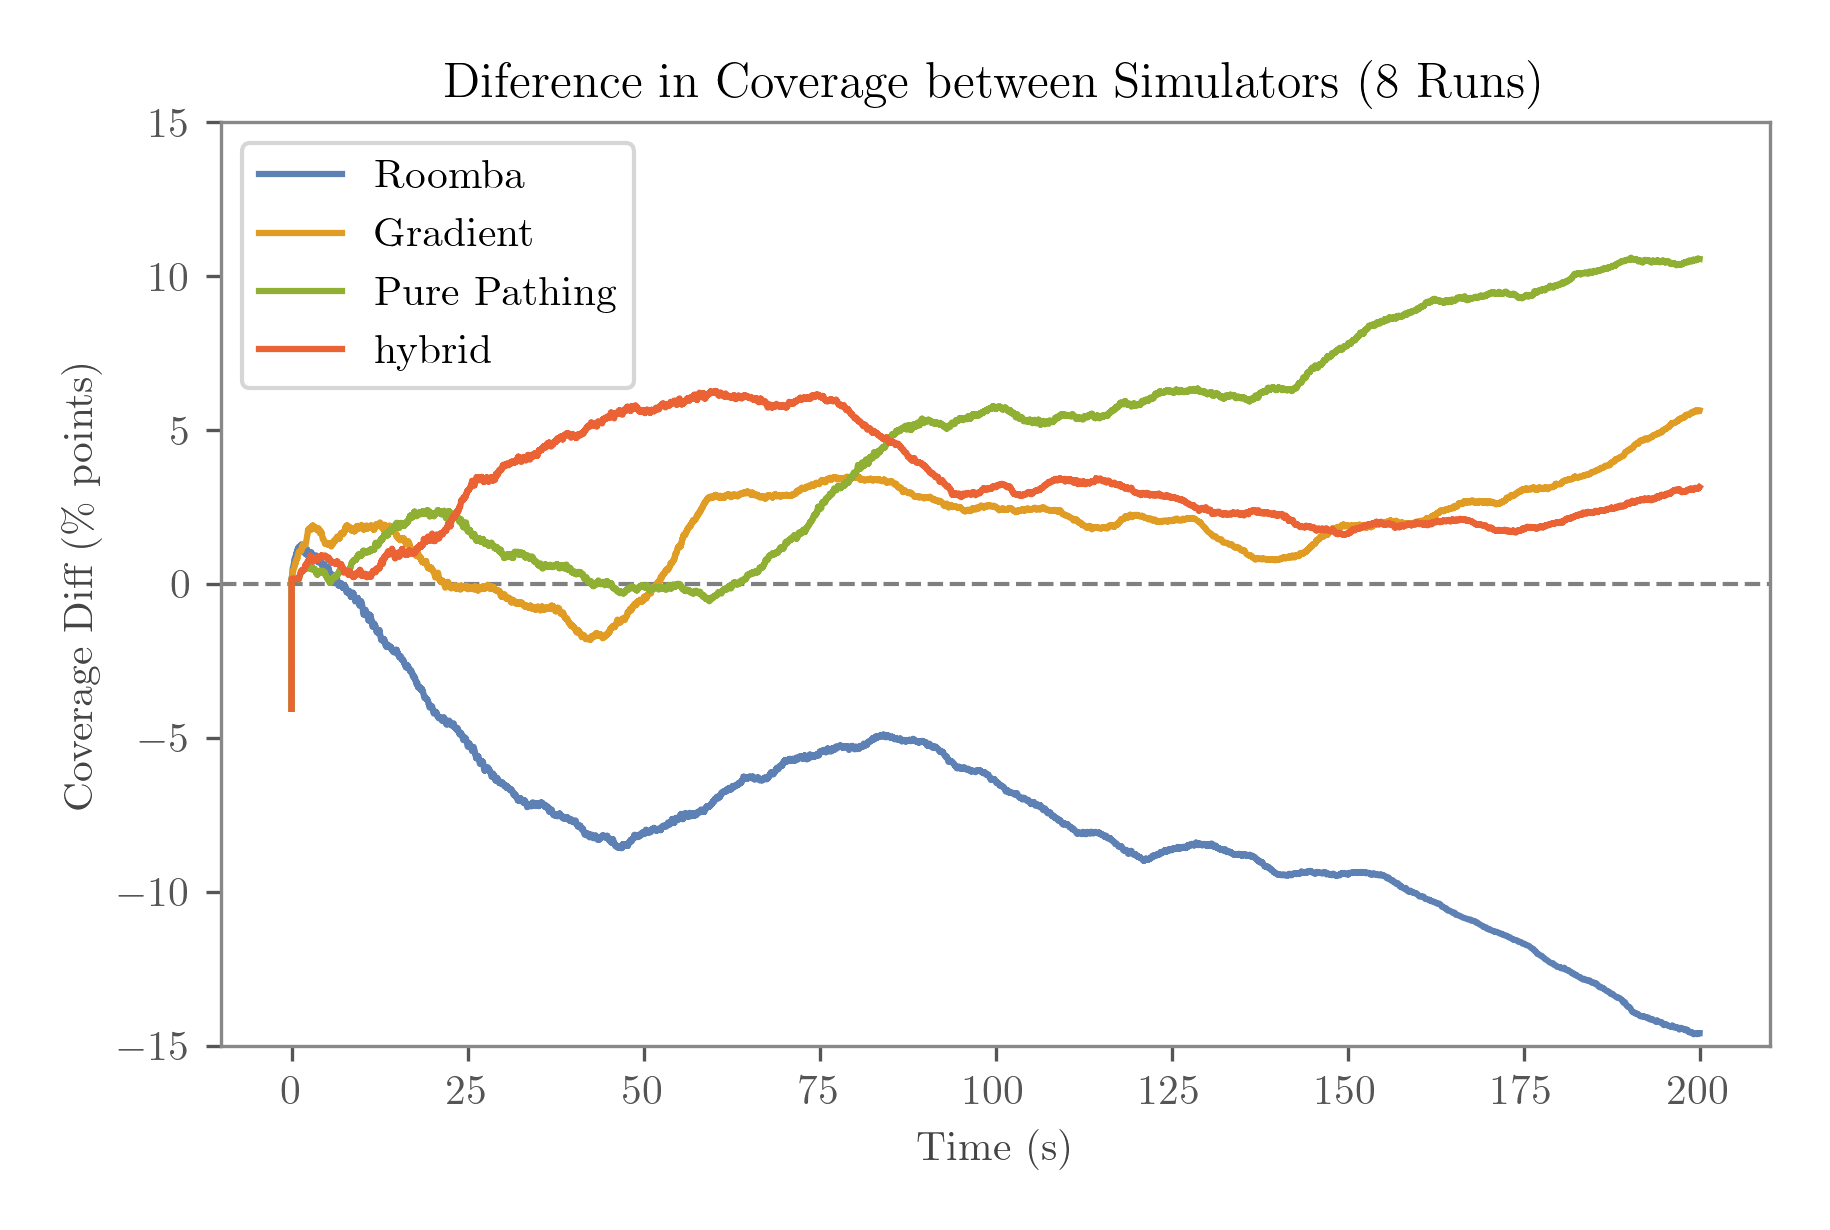
\includegraphics[width=0.90\textwidth]{./figures/plots/consistency/sim_coverage_diff.png}
    \end{center}
    \caption{Comparison of difference in coverage over time between ROS 2 Gazebo and \texttt{simple\_sim}.}
    \label{fig:coverage-benchmark-diff}
\end{figure}

\subsection{Search Algorithm Benchmarks}
\label{sec:search-algorithms-benchmark}
% TODO: Write duration of the trials (in text and figures)
Each algorithm was run 10 times on the Depot and Warehouse maps with 1, 2, 4, 8 robots using \texttt{simple\_sim}. The warehouse map was also run with 16 robots. The relative performance between the behaviors seems stable regardless of robot count. \Cref{fig:coverage-benchmark} shows a representative result with 4 robots.All results can be found in Appendix \ref{appendix:more-plots}. 


% TODO: Move common caption text to common caption
% TODO: Mention robot count
\begin{figure}[H]
  \centering
  \begin{subfigure}[b]{0.49\textwidth}
    \centering
    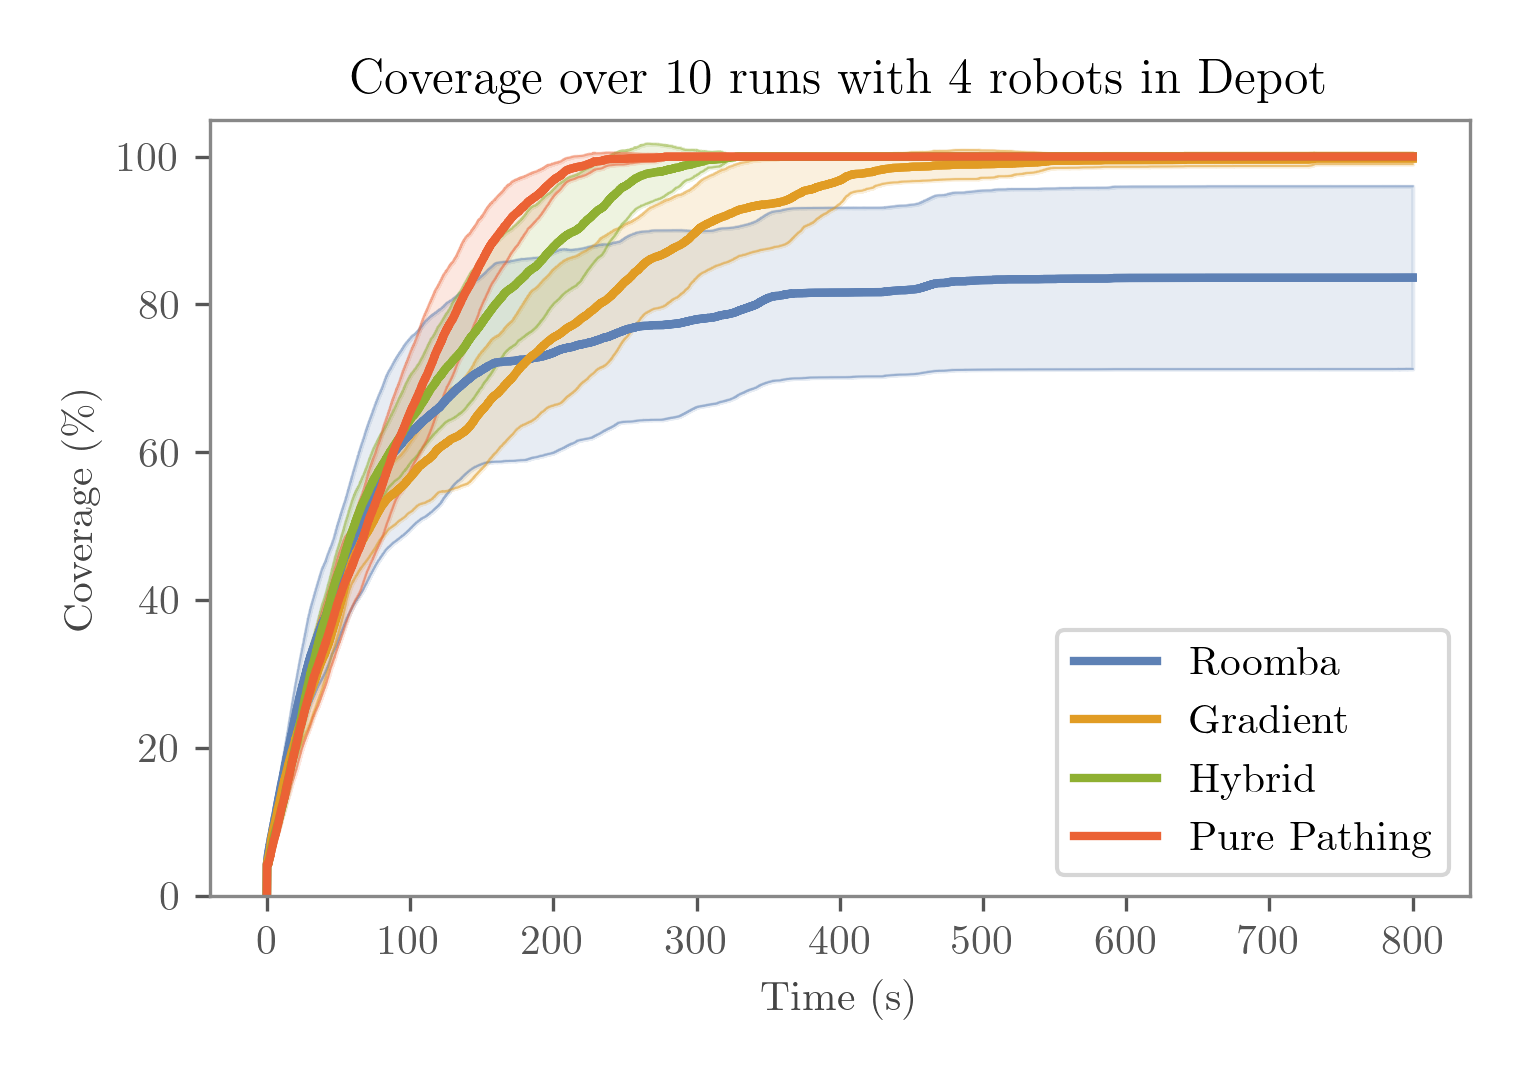
\includegraphics[width=\textwidth]{./figures/plots/benchmarks/coverage-over-10-runs-with-4-robots-in-depot.png}
      \caption{Results from running 4 robots in the Depot environment with \texttt{simple\_sim}.}
  \end{subfigure}
  \begin{subfigure}[b]{0.49\textwidth}
    \centering
    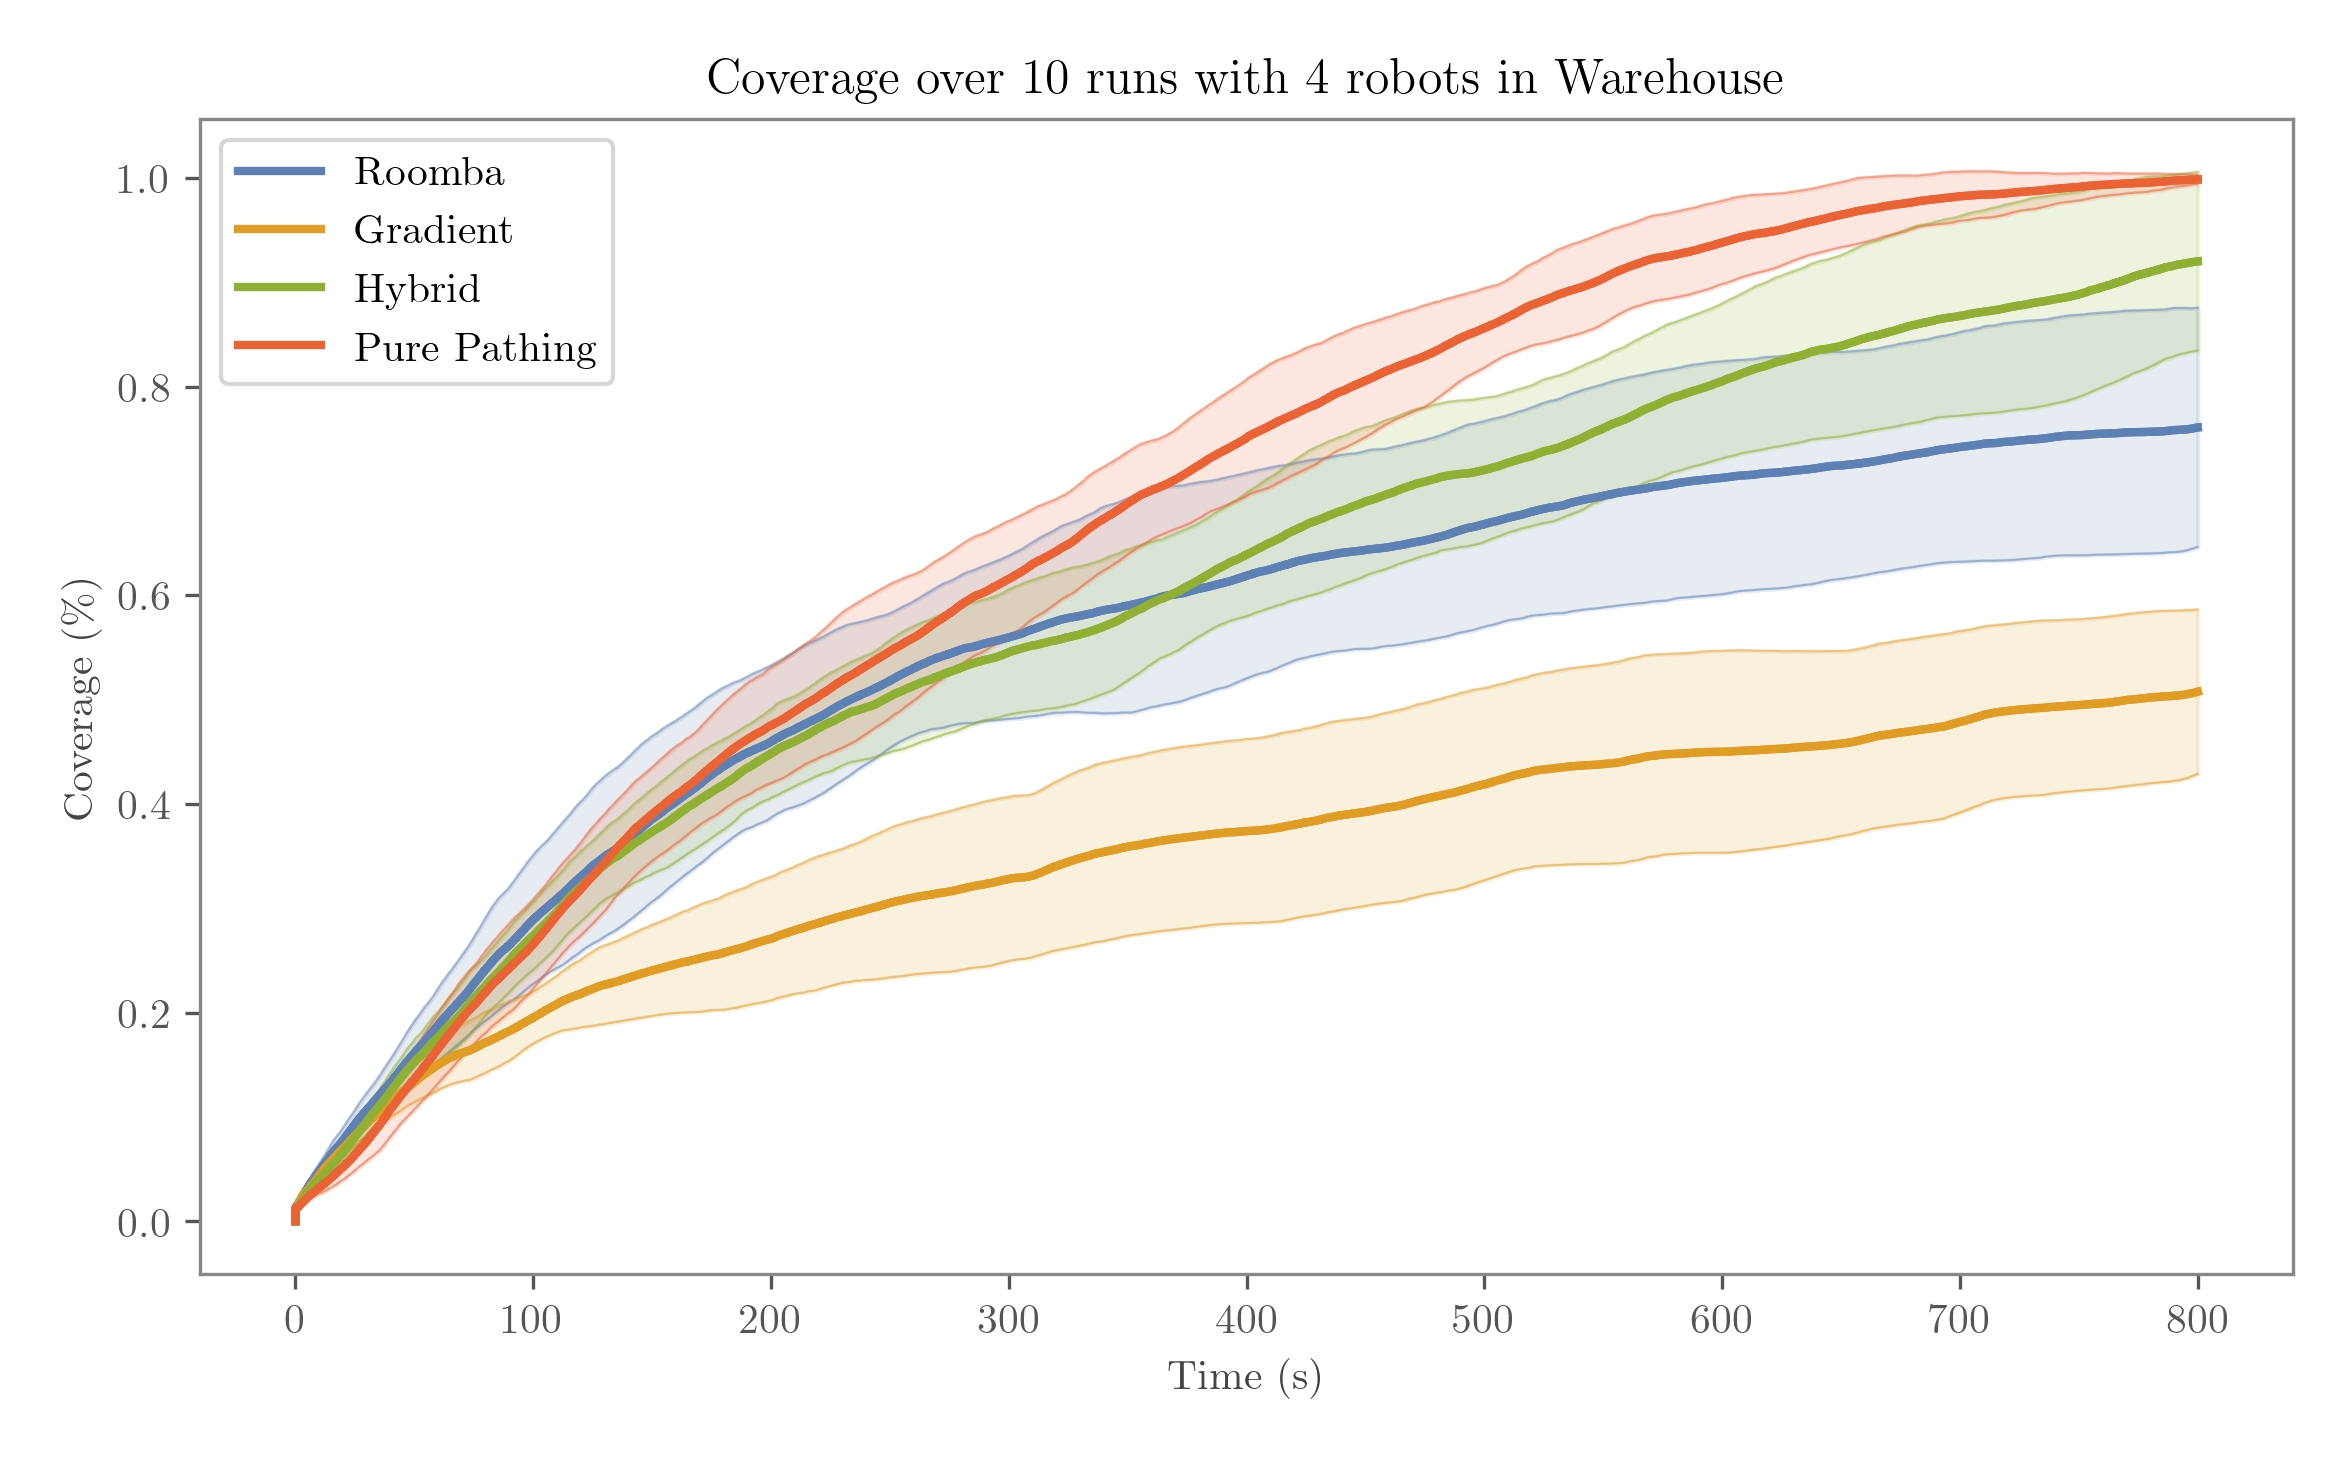
\includegraphics[width=\textwidth]{./figures/plots/benchmarks/coverage-over-10-runs-with-4-robots-in-warehouse.png}
      \caption{Results from running 4 robots in the Warehouse environment with \texttt{simple\_sim}.}
  \end{subfigure}
    \caption{Coverage performance of search algorithms over 10 runs starting in random positions in the same environment.}
    \label{fig:coverage-benchmark}
\end{figure}

The results clearly show that the Pure Pathing outperforms the other algorithms followed by the Hybrid algorithm. The Gradient algorithm is significantly worse than both the Pure Pathing and Hybrid algorithms. The Roomba algorithm is generally better performing in the beginning of the run, but has a hard time getting full coverage of the map, and is overtaken by the Gradient algorithm which has the search gradient to guide it towards unexplored areas.

% All algorithms eventually achieve full coverage, though their exploration efficiency varies significantly. 
% Gradient-based methods tend to cover local areas quickly but slow down due to diminishing gradients near fully explored zones. 
% Frontier-based methods achieve higher global efficiency by directing robots toward unknown regions, but at a higher computational cost. The hybrid method strikes a balance by switching strategies based on local exploration progress. 
% Deep reinforcement learning shows promise but requires further tuning for consistent early-stage performance.

\def\w{0.329\textwidth}
\begin{figure}[H]
    \centering
    \begin{subfigure}[b]{\w}
        \centering
        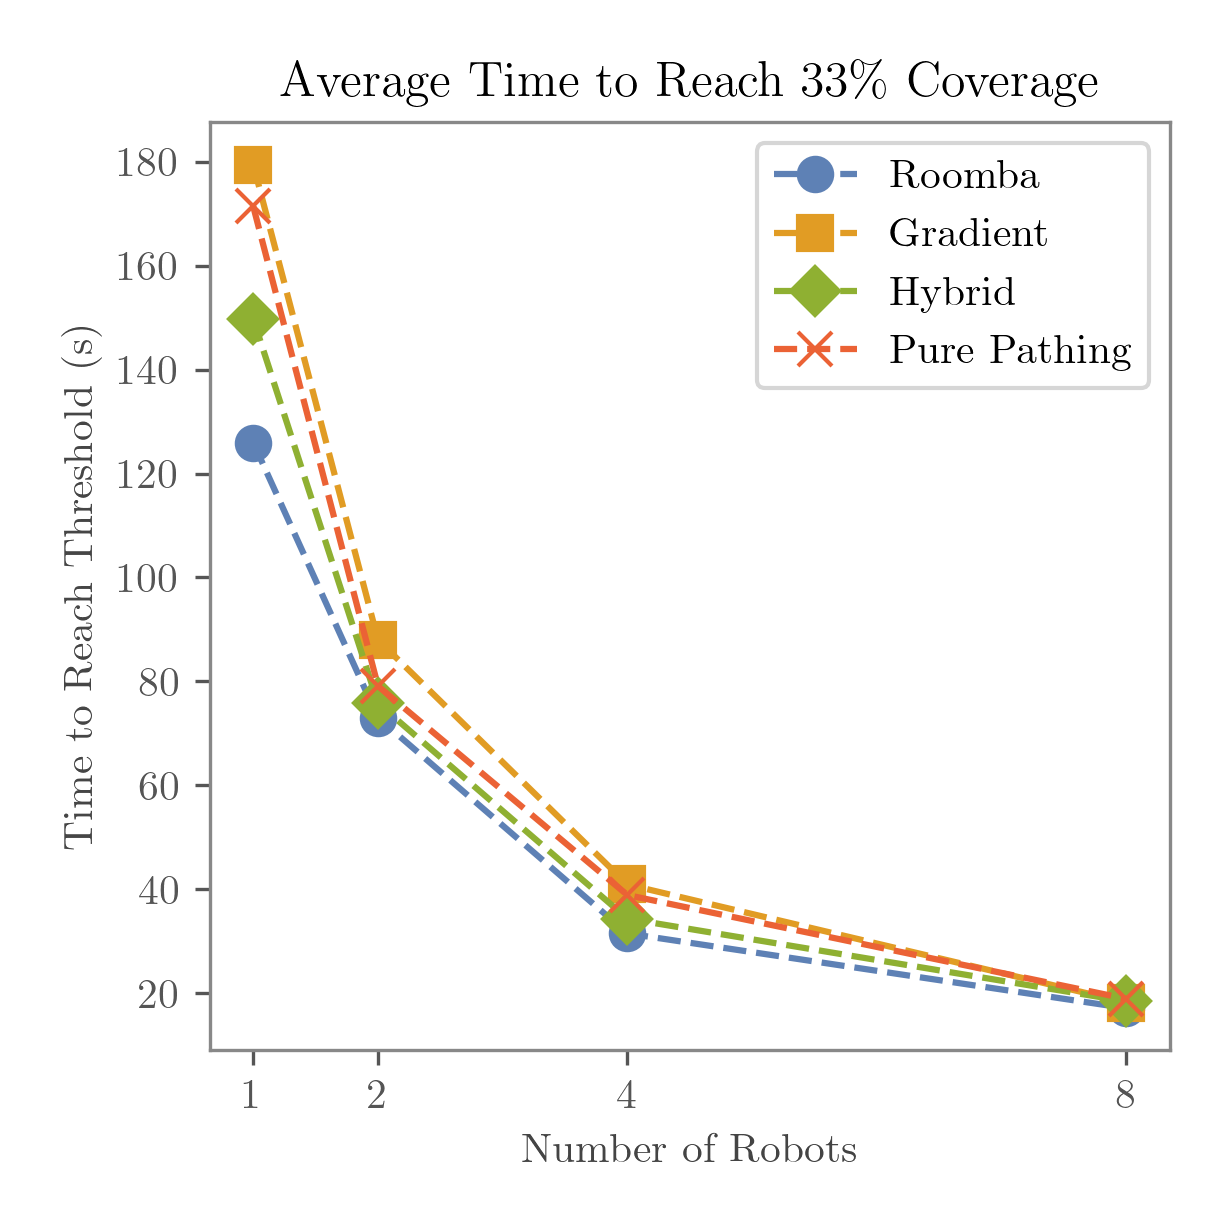
\includegraphics[width=\textwidth]{figures/plots/benchmarks/big-coverage-0.33-depot.png}
    \end{subfigure}
    \begin{subfigure}[b]{\w}
        \centering
        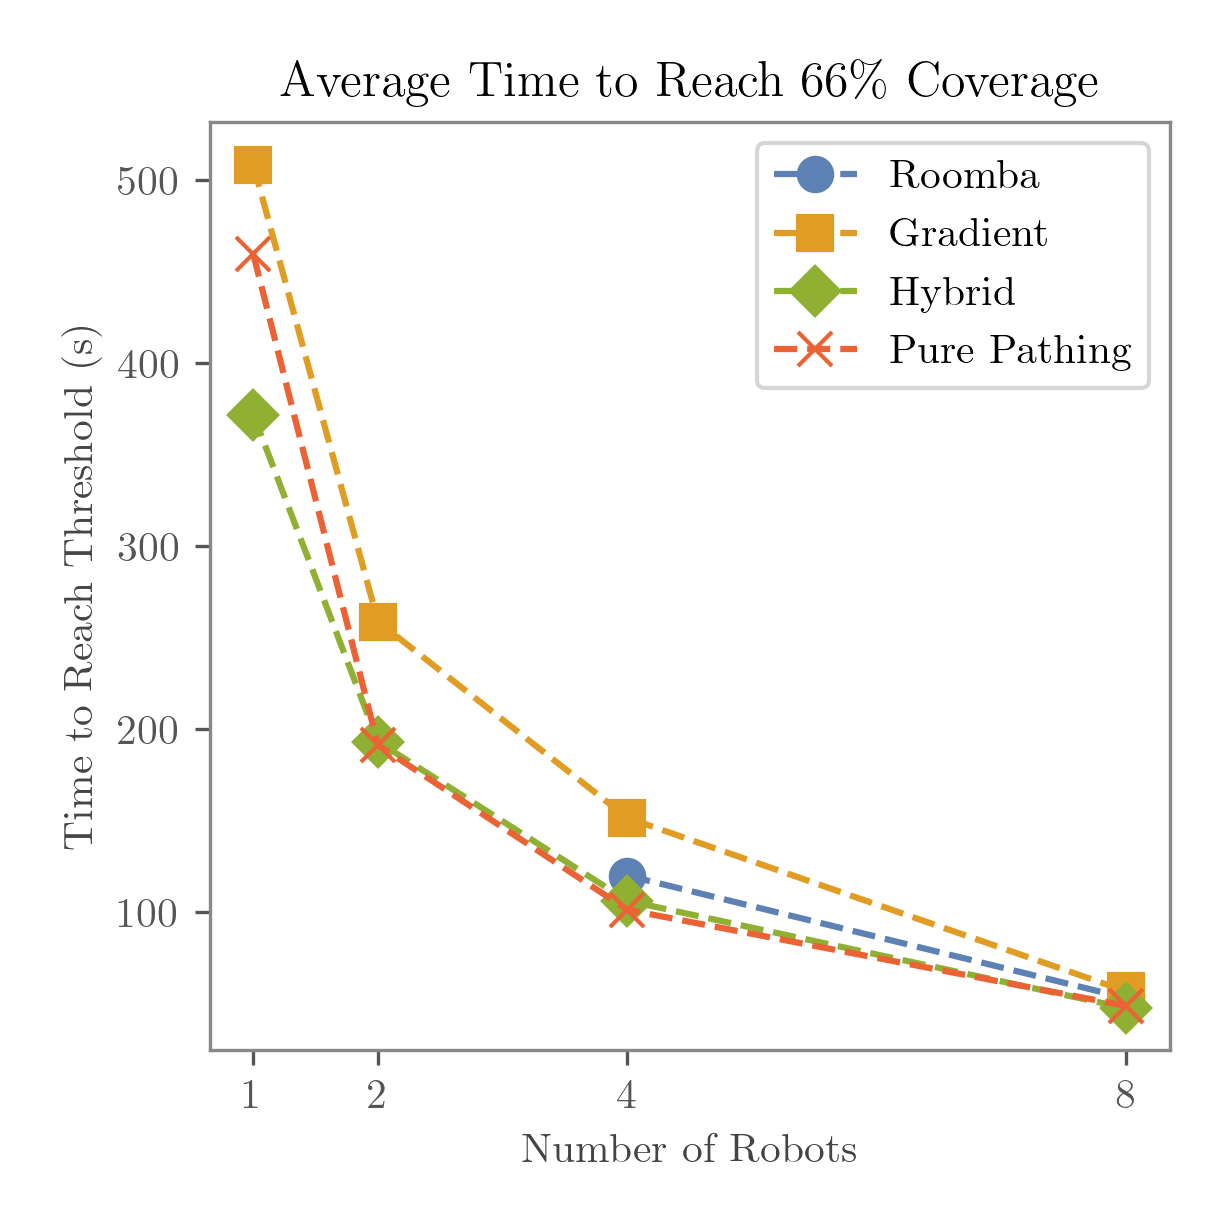
\includegraphics[width=\textwidth]{figures/plots/benchmarks/big-coverage-0.66-depot.png}
    \end{subfigure}
    \begin{subfigure}[b]{\w}
        \centering
        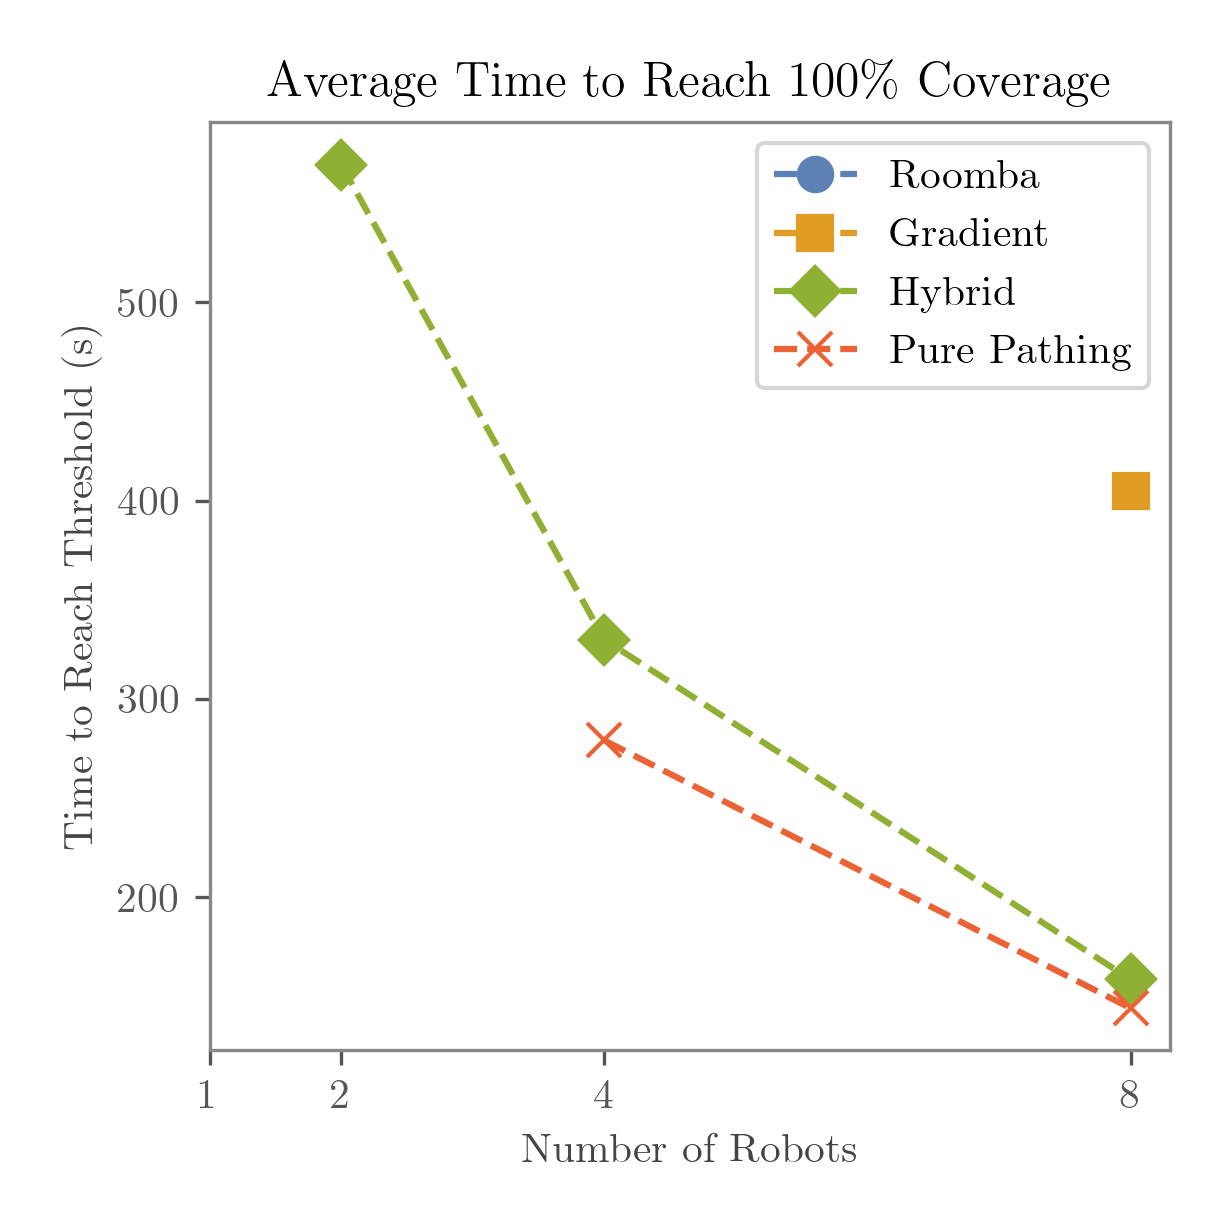
\includegraphics[width=\textwidth]{figures/plots/benchmarks/big-coverage-1.0-depot.png}
    \end{subfigure}
    \caption{Average time it takes the swarm to cover 33\%, 66\% and 100\% of the map in the Depot environment over 10 runs. Points are left out if the swarm did not reach these thresholds on average.}
    \label{fig:depot-threshold}
\end{figure}

\def\w{0.329\textwidth}
\begin{figure}[H]
    \centering
    \begin{subfigure}[b]{\w}
        \centering
        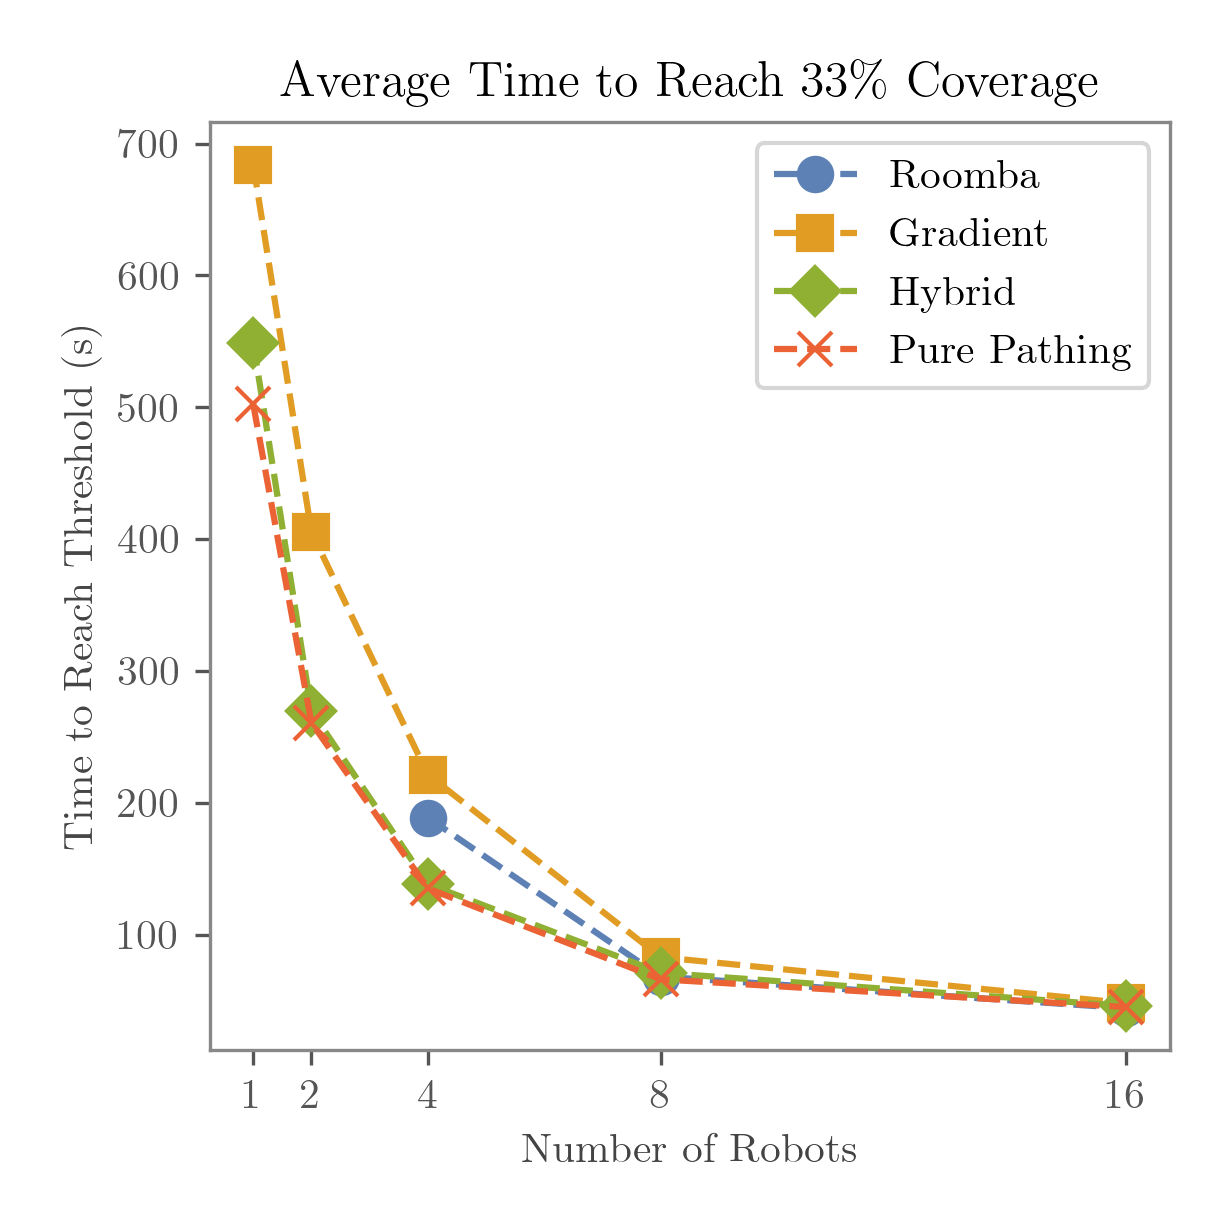
\includegraphics[width=\textwidth]{figures/plots/benchmarks/big-coverage-0.33-warehouse.png}
    \end{subfigure}
    \begin{subfigure}[b]{\w}
        \centering
        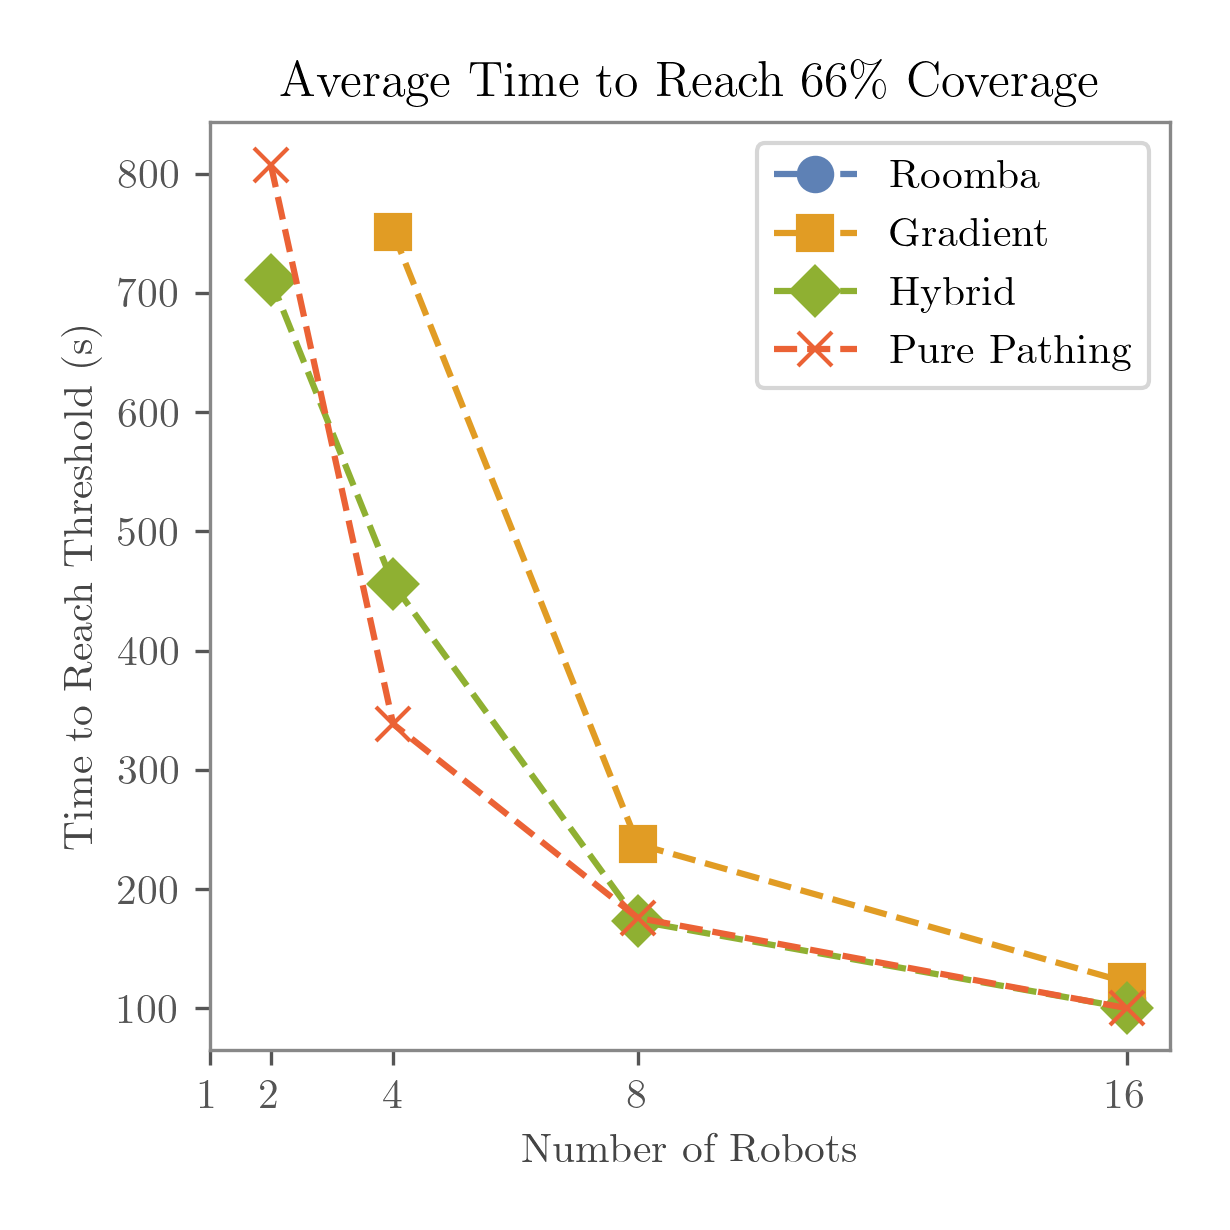
\includegraphics[width=\textwidth]{figures/plots/benchmarks/big-coverage-0.66-warehouse.png}
    \end{subfigure}
    \begin{subfigure}[b]{\w}
        \centering
        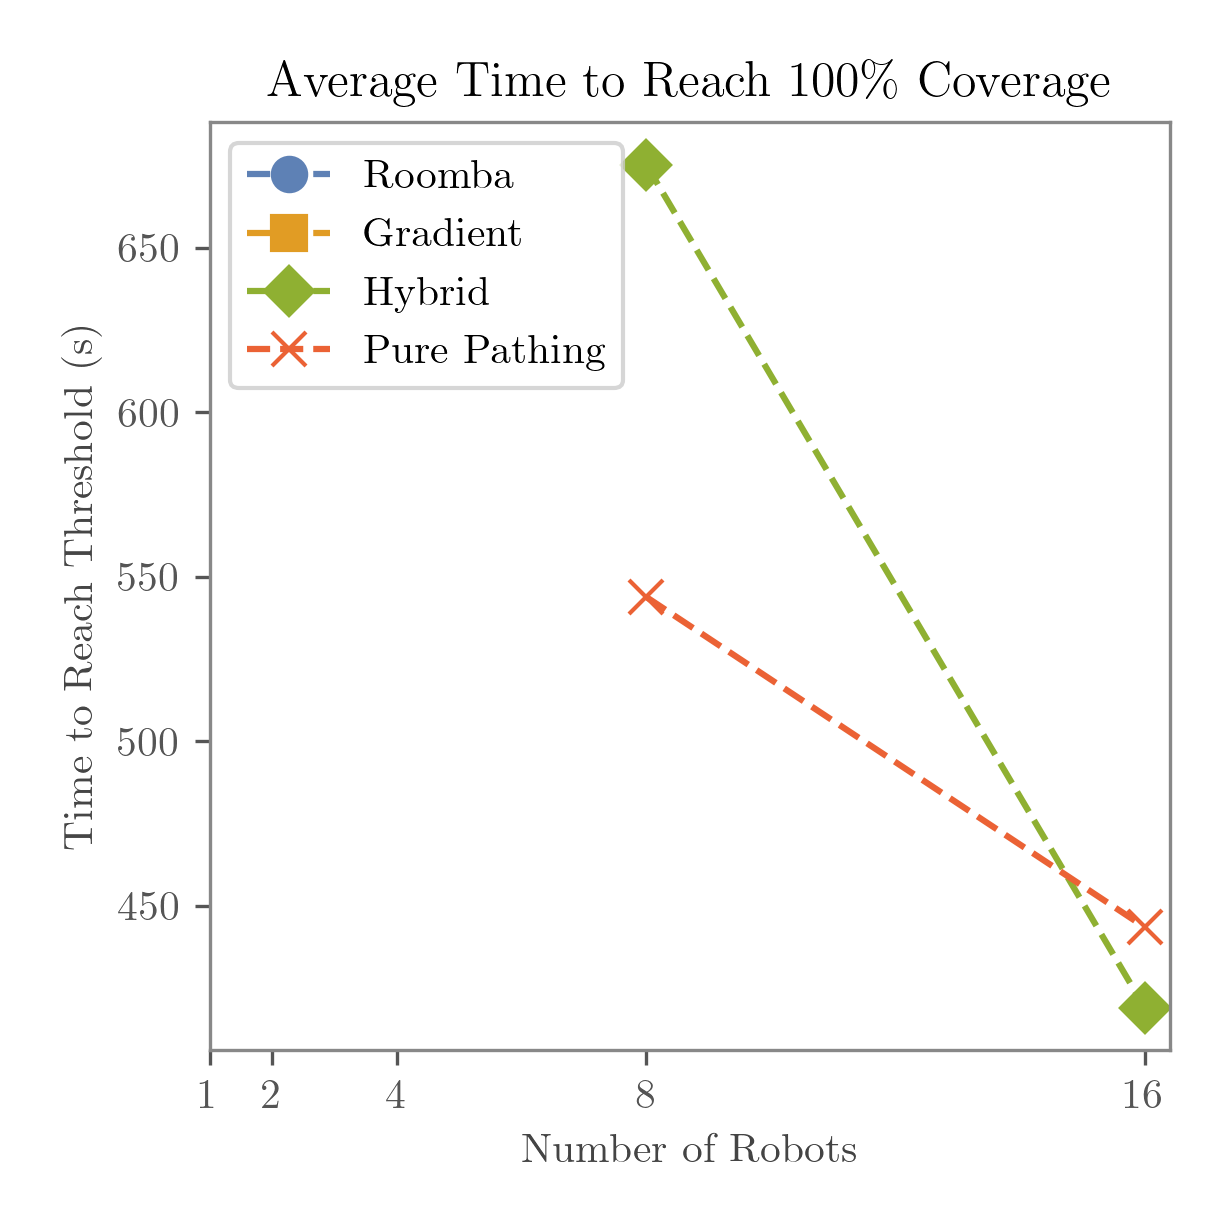
\includegraphics[width=\textwidth]{figures/plots/benchmarks/big-coverage-1.0-warehouse.png}
    \end{subfigure}
    \caption{Average time it takes the swarm to cover 33\%, 66\% and 100\% of the map in the Warehouse environment over 10 runs. Points are left out if the swarm did not reach these thresholds on average.}
    \label{fig:warehouse-threshold}
\end{figure}

% TODO: Maybe explain causes in discussion
\Cref{fig:depot-threshold} and \cref{fig:warehouse-threshold} show the average time it takes the swarm to cover different coverage thresholds of the map in the Depot and Warehouse environments, respectively with a varying number of robots. {\color{red} Here, it is clear that the Pure Pathing and Hybrid behaviors are able to use their global view of the map to find remaining unexplored regions.} It is also evident that the Roomba algorithm performance is drastically reduced in the more complex Warehouse environment as it never reaches above 33\% with any number of robots within the time span of the trial.

\subsection{Computational Performance}
A critical aspect of the search algorithm's performance is computational requirement for running the behaviors.

\subsubsection{Computation Time}
\Cref{fig:computation-performance} presents distributions of time to run the behavior in each time step. The benchmark was recorded over 6 runs for each algorithm running in the same environment. General observations are:

% TODO: Turn into paragraph
% TODO: Mention that pure pathing seems to be more computationally unstable. Sensitive to outliers. Effect on microcontrollers.
\begin{itemize}
  \item The \textbf{Roomba} algorithm, being the simplest, exhibits the lowest and most consistent computation time.
  \item The \textbf{Pure Pathing} algorithm also performs efficiently on average, though it shows more outliers due to the occasional expensive operations --- namely, costmap generation, frontier exploration/evaluation, and path planning --- which are not triggered at every time step.
  \item The \textbf{Gradient} method is consistent but is the slowest on average, as gradient recalculation occurs at each step.
  \item The \textbf{Hybrid} method was expected to fall between Pure Pathing and Gradient in terms of complexity as it uses a combination of the two. This assumption holds based on the observed data.
\end{itemize}

% TODO: Log scale mention
\begin{figure}[H]
    \begin{center}
        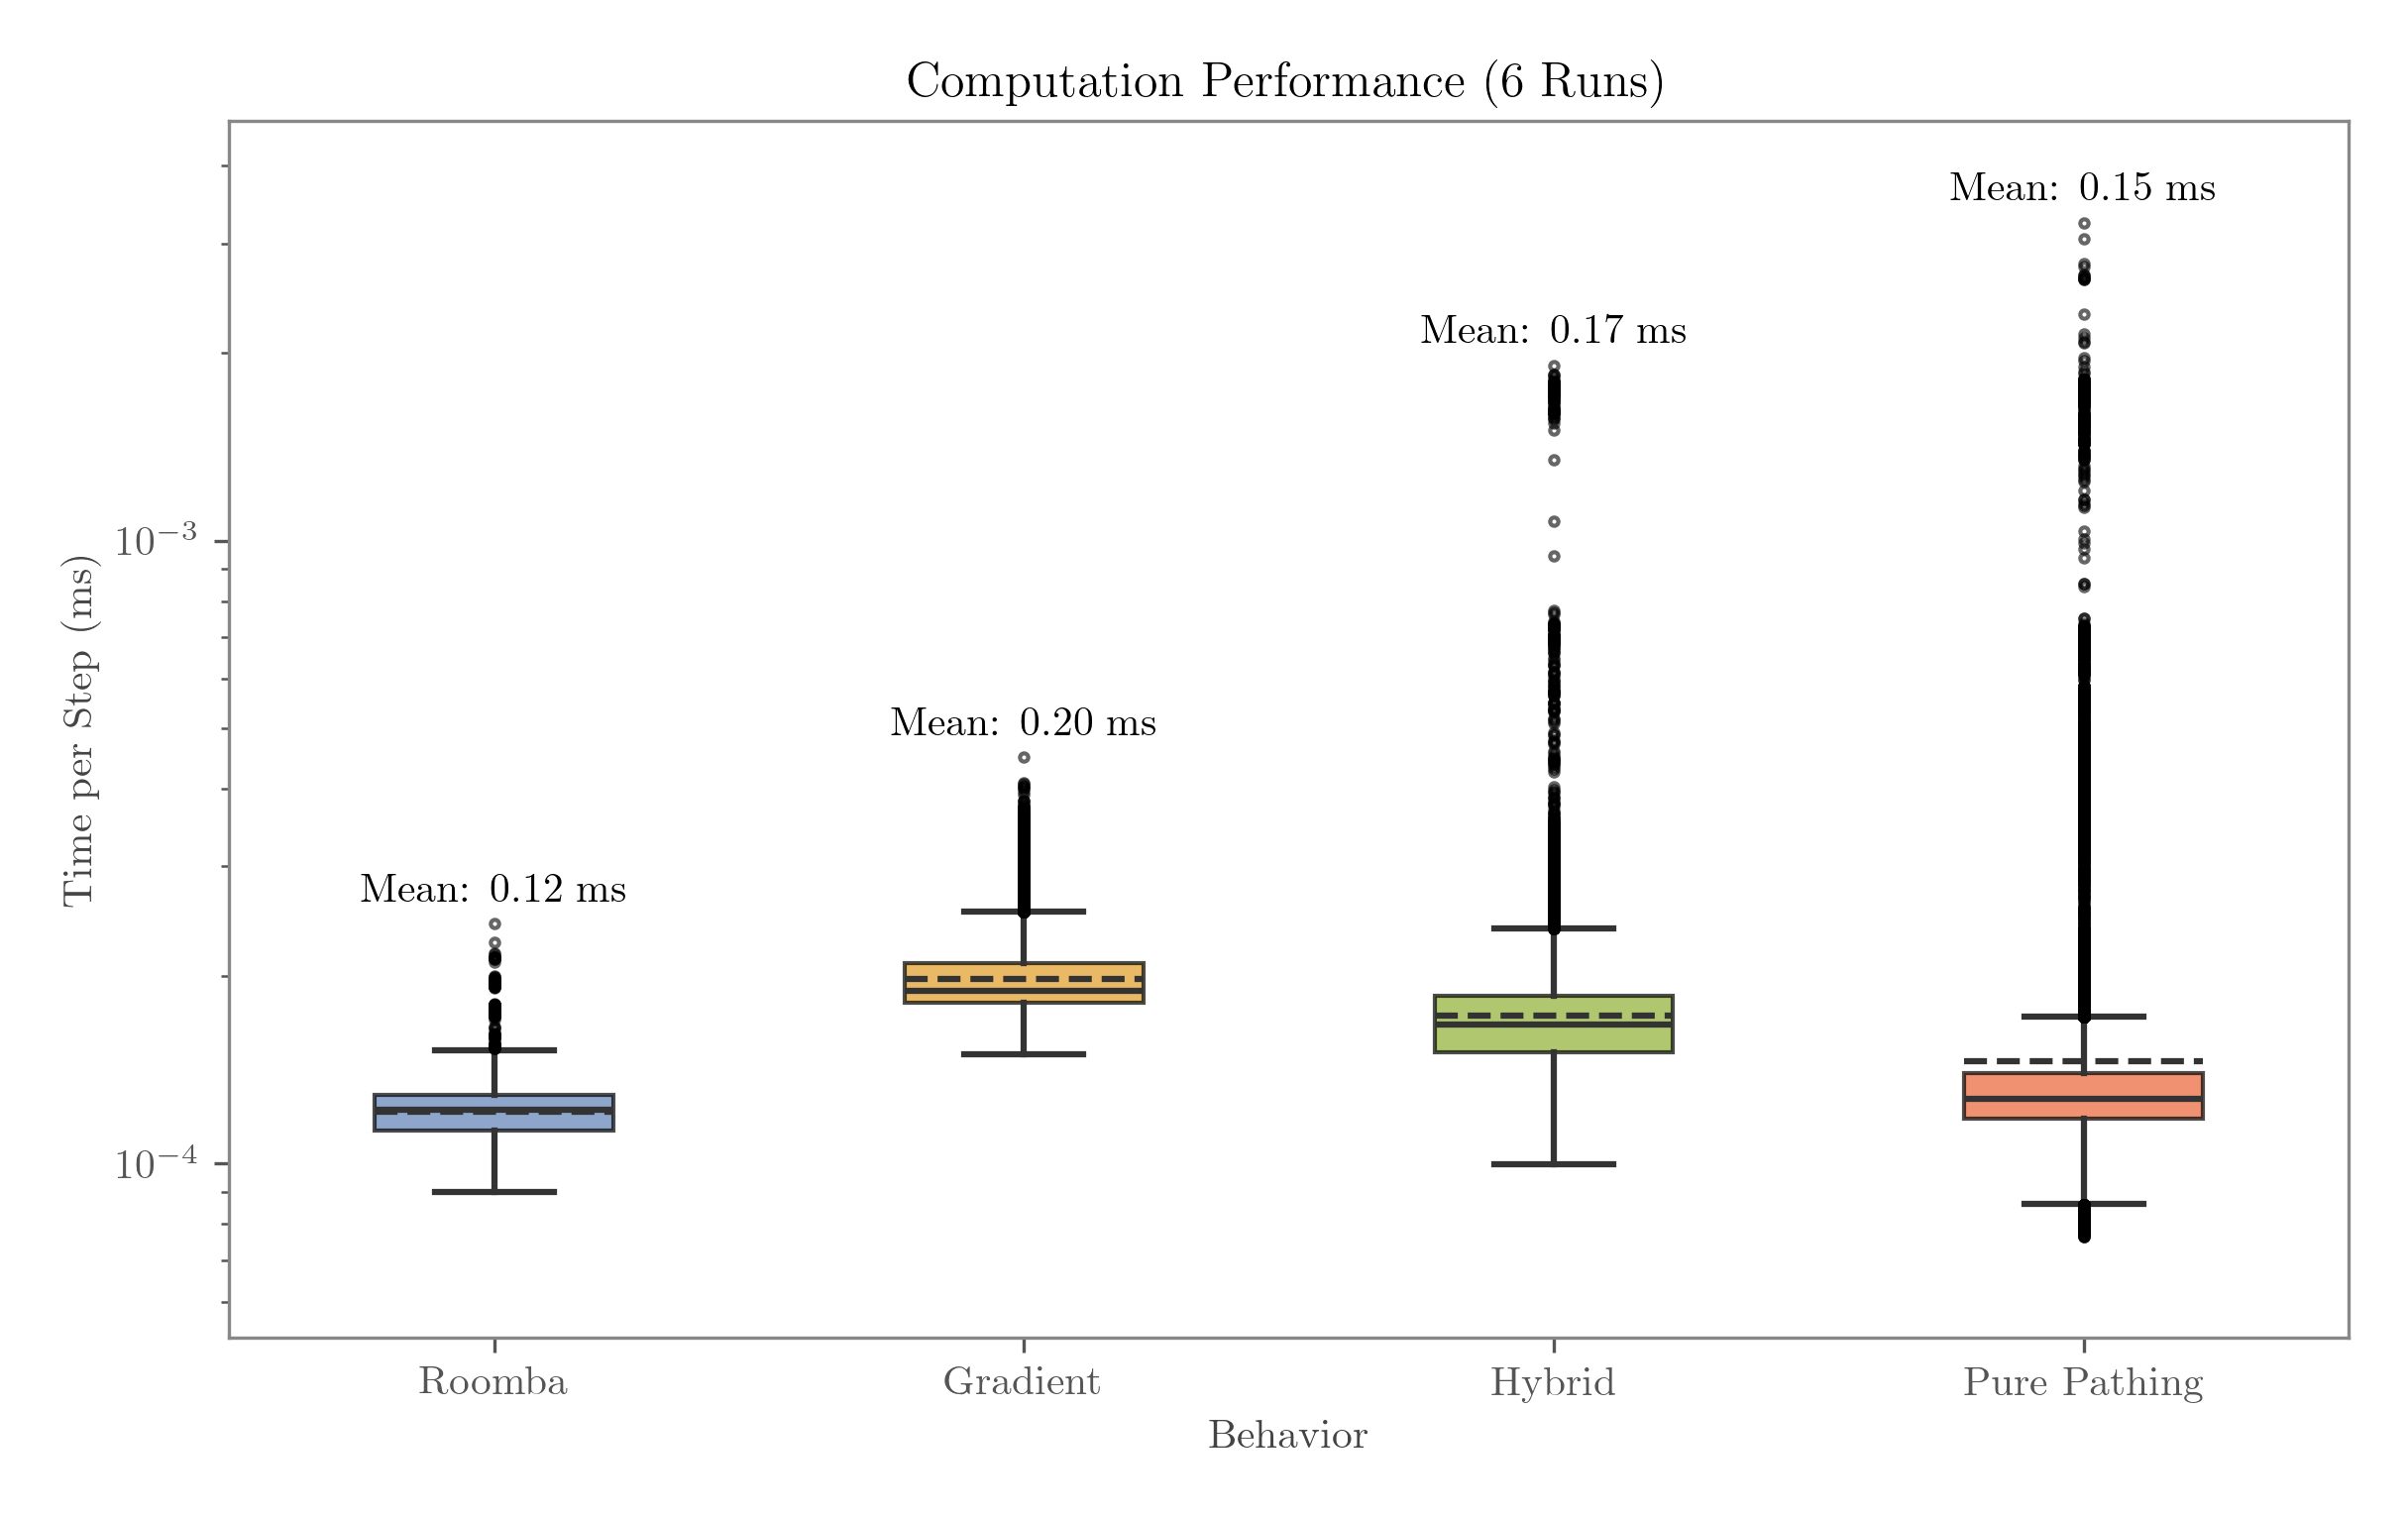
\includegraphics[width=0.95\textwidth]{./figures/plots/computation-performance-(6-runs).png}
    \end{center}
    \caption{Computation time for each search algorithm in the same map environment.}
    \label{fig:computation-performance}
\end{figure}

\subsection{Communication Load}
The messages transmitted during operation are updates to the search grid, which are sent whenever a robot’s internal search grid is modified. From these updates, other robots can synchronize their local search grids and infer the position of the robot that originated the message. Each message has a fixed size of 26 bytes. The \texttt{botbrain} library includes a configurable parameter that controls the broadcast frequency. The frequency is set to 10 Hz by default, which is one message every 100 ms, resulting in approximately 260 bytes/sec of outbound communication per robot. \\

% TODO: Maybe only mention this here and not in further development
A bandwidth of 260 bytes/sec negligible for most communicatino technologies considered for real-world deployment (see \cref{sub:communication-methods}), including Wi-Fi, Zigbee, and cellular. However, it may exceed practical limits for LoRa, particularly as the number of robots increases or in scenarios requiring higher message frequencies. If LoRa is to be considered for deployment, further message compression, reduced transmission frequency, or more aggressive filtering strategies would be necessary to meet the bandwidth constraints.

\subsection{Simulator Performance}
\label{sec:simulator-performance}
The performance and rapid iteration cycle offered by the \texttt{simple\_sim} simulator were key motivations for its development in this project. To quantify its efficiency, a simple benchmark was conducted by running both simulators headless (without a GUI) for 600 simulated seconds using the Roomba algorithm. Over 5 runs, Gazebo required 628 real-time seconds on average to complete the simulation, whereas \texttt{simple\_sim} completed the same task in an average of just 18 seconds. This substantial difference highlights the lightweight simulator’s superior computational performance.

The ability to run simulations significantly faster than real time is highly beneficial for development. It enables rapid experimentation, easier debugging, and efficient benchmarking of algorithmic changes—making \texttt{simple\_sim} a preferable tool during the design and testing phases.

\subsubsection{Gazebo Stability}
Benchmark data was collected with Python scripts which run both \texttt{simple\_sim} and Gazebo on the same environments automatically for a set of runs. Gazebo was, however, quite unreliable in its initialization which meant that Gazebo had to be supervised during benchmarking. This made it infeasible to run long trials multiple times with multiple behaviors. The following sections contain plots with data gathered using \texttt{simple\_sim} and would have taken days of supervised benchmarking to record using Gazebo.

